\chapter{On Graphs, Feature Structures and Systemic Networks}
\label{ch:data-structures}
%graphs, graph patterns, attribute-value matrices etc.\\ what can they do?

%\section{Introduction}
%\menote*{Rewrite}{
%In this section I present a method to generate mood constituency graph together with more general graph properties and operations over them. The Stanford Dependency Schema proposed by \citet{Marneffe2006} and re-motivated latter in \citeyearpar{Marneffe2008} constitutes the departing point of the current approach in building a  Mood Constituency Graph (MCG). MCG is the structure reflecting mood analysis(described in chapter \ref{}) and serves as the backbone for performing transitivity analysis(described \ref{}) via Graph Matching operations. The method involves three types of graph structures: (1) Dependency Graphs, (2) Mood Constituency Graphs and (3) Pattern Graphs. 
%
%In the following I first introduce the specifics of a generic graph structure and the operations that these graphs support and then we present the parsing algorithms. 
%}
%{\tiny }
%The parsing algorithm does not operate on free text but uses a dependency parser (in this case Stanford Dependency Parser \cite{}) bootstrapping the process with a DG backbone.

The parsing algorithm, whose pipeline architecture we have seen in Section \ref{sec:architecture}, operates mainly with operations on graphs, attribute-value matrices and ordered lists with logical operators. This chapter defines the main types of graphs, their structure and how they are used in the following chapters which detail on the parsing process. This chapter also covers the operations relevant to the parsing algorithm: \textit{conditional traversal and querying} of nodes and edges, \textit{graph matching}, \textit{pattern-graph matching} and \textit{pattern-based node selection, insertion and update}.

While developing the Parsimonious Vole parser a set of representational requirements arose that can be summarised as follows:

\begin{itemize}
	\item graphic representation 
    \item arbitrary relations (i.e. typed and untyped edges)
	\item description rich (i.e. features of nodes and edges)
	\item linear ordering and configurations (i.e. syntagmatic and compositional)
	\item hierarchical tree-like structure (with a root node) but also orthogonal relations among siblings and non-siblings
	\item statements of absence of a node or edge (i.e. negative statements in pattern graphs)
	\item disjunctive descriptions (handling uncertainty)
	\item conjunctive descriptions (handling multiple feature selections)
	\item (conditional) pattern specifications (i.e. define patterns of graphs)
	\item operational pattern specifications (i.e. a functional description to be executed in pattern graphs)
\end{itemize}

The general approach to construct an SFG parse structure revolves around the graph pattern matching and graph traversal. In the following sections I present the instruments used for building such structures, starting from a generic computer science definition of graphs and moving towards specific graph types covering also the feature structures and conditional sets. 

\section{On sets, feature structures and graphs}
\label{sec:graphs}

In the field of computational linguistics trees has been taken as the de facto data representation. In Section \ref{sec:paradigmatic-account} I have mentioned already that I employ graph and not tree structures. 

Firstly, the trees are a special kind of graphs. Anything expressed as a tree is as well a tree. Secondly, we gain a higher degree of expressiveness even if at the expense of computational complexity, a point to which we will come back latter in Section \ref{sec:graph-matching}. This expressiveness is needed when dealing with interconnection of various linguistic theories which in practice is done by mapping the nodes of one tree structure onto the nodes of another one. In addition, the structures are not always trees. There are situations when a node has more than one parent or when a node is connected to its siblings which break the tree structure. 

\begin{definition}[Graph]\label{def:graph}
	A \textit{graph} $G=(V,E)$ is a data structure consisting of non-empty set $V$ of nodes and a set $E\subseteq V \times V$ of edges connecting nodes.
\end{definition}

\begin{definition}[Digraph]\label{def:digraph}
	A \textit{digraph} is a graph with directed edges. A directed edge $(u,v)\in E$ is an ordered pair that has a start node $u$ and an end node $v$ (with $u, v \in V$)
\end{definition}

%A directed graph is a set of objects called nodes some of which are connected in pairs by directed links called edges. The nodes are feature structures or are objects described by a feature structure while the edges are represented as triples \textit{(x,y,f)} where \textit{x} and \textit{y} are the connected nodes and \textit{f} is the feature structure of the edge.

In this thesis the graph nodes are considered to be \textit{feature structures} forming \textit{Feature Rich Graphs} (see Definition \ref{def:feature-rich-graph}). Before formally defining these graphs, I need to address first the notion of feature structure and a few kinds of sets. 

In SFL the concept of \textit{feature} takes up an important role. Also features are said to form systems of choices that are structured in relation to one another and are suitable for describing linguistic objects and phenomena.

\citet{Pollard1987} have formally described useful concepts for grammatical representations in the context of Head-Driven Phrase Structure Grammar (HPSG). He adopts the \textit{typed feature structure theory} and extends it in ingenious ways applicable in computational linguistics. Among others, he provides formal definitions for the concepts of \textit{feature structure}, \textit{hierarchy}, \textit{logical evaluation}, \textit{composition} and \textit{unification}, the latter, being key operations in parsing using feature structured grammars. 

In this thesis, feature structures are important but only in a simplified version serving as graph node descriptions. The main reason is the difference in approach as the main parsing operations, here, are based on graph pattern matching (introduced in the sections below).

In a broad computer science sense, including Pollard's definition, feature structures are equivalent to graph structures. So any feature structure can be expressed as a graph and any graph can be expressed as a feature structure. But in a narrow sense, as adopted in this thesis, it is useful to employ both concepts but each for a given purpose. The feature structure is reduced to an attribute-value matrix (see Definition \ref{def:fs}) and the graphs to a network of feature structure nodes (see Definition \ref{def:feature-rich-graph}) i.e. no atomic nodes.

\begin{figure}[!ht]
    \centering
    \begin{subfigure}[b]{0.5\textwidth}
        \centering
        \begin{tikzpicture}[node distance=1.2em, scale=0.85, transform shape]
        \node[pattern-node, anchor=center,] (n1) {Node 1 \\ $\begin{Bmatrix}
            f_1: & v_1 \\
            f_2: & v_2 \\
            f_3: & v_3 \\
            \end{Bmatrix}$};
        \node[pattern-node, anchor=center, below=6em of n1] (n2) {Node 2 \\ $ \begin{Bmatrix}
            f_5: & v_5 \\
            f_6: & v_6 \\
            f_7: & v_7 \\
            \end{Bmatrix}$};
        \draw[sequence,->] (n1) -- (n2);
        \end{tikzpicture}
        \caption{The graph with feature structure nodes}
        \label{fig:example-graph-compact1}
    \end{subfigure}%
    \begin{subfigure}[b]{0.5\textwidth}
        \centering
        \begin{tikzpicture}[node distance=1.2em, scale=0.85, transform shape]
        \node[pattern-node, anchor=center,] (n1) {Node 1};
        \node[pattern-node, anchor=center, below=2.7em of n1] (n2) {Node 2};
        
        \node[pattern-node, anchor=center, above=3em of n1,xshift = -3em ] (n1f1) {$v_1$};
        \node[pattern-node, anchor=center, above=3em of n1,xshift = 0em ] (n1f2) {$v_2$};
        \node[pattern-node, anchor=center, above=3em of n1,xshift = 3em] (n1f3) {$v_3$};
        
        \node[pattern-node, anchor=center, below=3em of n2,xshift = -3em] (n2f4) {$v_4$};
        \node[pattern-node, anchor=center, below=3em of n2,xshift = 0em] (n2f5) {$v_5$};
        \node[pattern-node, anchor=center, below=3em of n2,xshift = 3em] (n2f6) {$v_6$};
        
        
        \draw[sequence,->] (n1) -- (n2);
        \draw[sequence,->] (n1) -- (n1f1) node [midway, right=0em, ]{$f_1$};
        \draw[sequence,->] (n1) -- (n1f2) node [midway, right=0em, ]{$f_2$};
        \draw[sequence,->] (n1) -- (n1f3) node [midway, right=0em, ]{$f_3$};
        
        \draw[sequence,->] (n2) -- (n2f4) node [midway, right=0em, ]{$f_4$};
        \draw[sequence,->] (n2) -- (n2f5) node [midway, right=0em, ]{$f_5$};
        \draw[sequence,->] (n2) -- (n2f6) node [midway, right=0em, ]{$f_6$};
        
        \end{tikzpicture}
        \caption{The graph with atomic nodes}
        \label{fig:example-graph-compact2}
    \end{subfigure}%
    \caption{Graphs with atomic nodes and feature structure nodes}
    \label{fig:example-graph-compact}
\end{figure}

The main reasons in this separation are efficiency and practicality. First, it is about handling the atomic values (strings or integers) and (ordered) arrays only as values of feature structures and never as graph nodes. Second, the graphs remain limited in size, close to the conceptualised linguistic structures, i.e. dependency or constituency. Otherwise, the graphs would grow in complexity (a) by at least one more round of nodes for each dependency or constituency node and (b) by adoption of an additional node classification.

For example lets imagine a constituency graph fragment of two nodes \textit{Node 1} and \textit{Node 2} where each has three associated features as it can be seen in Figure \ref{fig:example-graph-compact1}. If we would insist to dispose of the feature structure within the node and express the features as atomic graph nodes then the result would be a graph structure such as the one in Figure \ref{fig:example-graph-compact2}.

\begin{definition}[Feature Structure (FS)]\label{def:fs}
	A \textit{feature structure} $F$ is a finite set of attribute-value tuples $f_{i} \in F$. A \textit{feature} $f=(a,v)$ is an association between an identifier $a$ (a symbol) and a value $v$ which is either an atomic value (symbol, number, string), a set or another feature structure. 
\end{definition}

The values of feature structures may be other feature structures allowing, if needed, to construct hierarchical descriptions. In the current implementation, however, the values of the feature structure are restricted to atomic values or sets of values.

For convenience I define two functions to access the identifier and value in a feature structure. The function $name:F \rightarrow symbol$ returns the feature symbol (identifier) $name(f)=a$ and the function $val:F \rightarrow \{atomic, Set, FS\}$ is a function returning the ascribed value of a feature $val(f)=v$. 

Definition \ref{def:fs} stipulates that the value of a feature may be also a set (besides an atomic value). The sets used in this thesis need to carry additional properties required for their interpretation. Specifically, it is the order need to be addressed here and the capacity to specify that set elements stand in a certain logical relation one to another (e.g. conjunction, disjunction, negation, etc.). These two properties are covered in Definition \ref{def:set} and \ref{def:conj-set}.
For convenience I will assume from now on that sets (see Definition \ref{def:set}) preserve order even when it is not really required.  

\begin{definition}[Set]\label{def:set}
	An (ordered) \textit{set} $S=\{o_1,o_2,...,o_n\}$ is a finite well defined collection of distinct objects $o_{i}$. A set is said to be ordered if the objects are arranged in a sequence such that $\forall o_{i-1},o_{i} \in S: o_{i-1}<o{i}$.
\end{definition}

\begin{definition}[Conjunction Set]\label{def:conj-set}
	A \textit{conjunction set} $S_{conj}=(S,conj)$ is a set $S$ whose interpretation is given by the logical operand $conj$ (also denoting the type of the set) such that $\forall o_{i},o_{j} \in S: conj(o_{i}, o_{j})$ holds.
\end{definition}

The conjunction sets used in current work are \textit{AND-set} ($S_{AND}$), \textit{OR-set} ($S_{OR}$), \textit{XOR-set} ($S_{XOR}$) and \textit{NAND-set} ($S_{NAND}$). The assigned logical operands play a role in the functional interpretation of conjunction sets. % such that for example a $S_{AND}$ set $T_1={a,b,c}$ is interpreted as the logical conjunction $a \wedge b \wedge c$. 
Formally these sets are defined as follows.

\begin{definition}[Conjunctive set]\label{def:and-set}
  Conjunctive set (also called \textit{AND-set}) is a conjunction set $S_{AND}=\{a,b,c...\}$ that is interpreted as a logical conjunction of its elements $a \wedge b \wedge c \wedge ...$ 
\end{definition}

\begin{definition}[Negative conjunctive set]\label{def:nand-set}
	Negative conjunctive set (also called NAND-set) is a conjunction set $S_{NAND}=\{a,b,c...\}$ that is interpreted as a negation of the logical conjunction of its elements $a \uparrow b \uparrow c \uparrow ...$ equivalent to $ \neg(a \wedge b \wedge c \wedge ...)$ 
\end{definition}

\begin{definition}[Disjunctive set]\label{def:or-set}
	Disjunctive set (also called OR-set) is a conjunction set $S_{OR}=\{a,b,c...\}$ that is interpreted as a logical disjunction of its elements $a \vee b \vee c \vee ...$
\end{definition}

\begin{definition}[Exclusive disjunctive set]\label{def:xor-set}
	Exclusive disjunctive set (also called XOR-set) is a conjunction set $S_{XOR}=\{a,b,c...\}$ that is interpreted as a logical exclusive disjunction of its elements $a \bigoplus b \bigoplus c \bigoplus ...$ equivalent to $ (a \wedge \neg (b \wedge c \wedge ... )) \vee (b \wedge \neg (a \wedge c \wedge ...)) \vee (c \wedge \neg (a \wedge b \wedge ...)) $
\end{definition}

When conjunction sets are used as values in FSs then the logical operand dictates the interpretation of the FS. When the set type is $S_{AND}$ then all the set elements hold simultaneously as feature values. If it is a $S_{OR}$ then one or more of the set elements hold as values. If is $S_{XOR}$ then one and only one of set elements holds and finally if it is a $S_{NAND}$ set then none of elements hold as feature values.

The function $\tau(S)$, defined $\tau:S \rightarrow \{S_{AND},S_{OR},S_{XOR},S_{NAND} \}$, returns the type of the conjunction set and the function $size(S)$, defined $size:S \rightarrow \mathbb{N}$, returns the number of elements in the set. The size function is also denoted as $|S|$.
 
Now that all the necessary basic notions nave been formally defined I now define the feature rich graph and provide a couple of examples afterwards. 
 
\begin{definition}[Feature Rich Graph (FRG)]\label{def:feature-rich-graph}
	A \textit{feature rich graph} is a digraph whose nodes $V$ are feature structures and whose edges $(u,v,f) \in E$ are three valued tuples with $ u,v \in V$ and $f \in F$ an arbitrary feature structure.
\end{definition}

Further on, for convenience, when I refer to a graph I will refer to a feature rich digraph unless otherwise stated. The parsing algorithm operates with such graph and they are further distinguished, based on purpose as: \textit{Dependency Graphs} (DG) (example figure \ref{fig:dep-graph}), \textit{Constituency Graphs} (CG) (example figure \ref{fig:mcg-graph}) and Pattern Graphs (PG) also referred as \textit{Query Graphs} (QG).

Please note that the edges are defined to carry feature structures. This capacity will not be employed, for example, in the case of constituency graphs; only minimally employed in the case of dependency graphs, where the dependency relation is specified; and fully employed in pattern graphs. Nonetheless, treating all of them as feature rich graphs simplifies the implementation.

\begin{definition}[Dependency Graph]\label{def:dep-graph}
	A \textit{dependency graph} is a feature rich digraph whose nodes $V$ correspond to words, morphemes or punctuation marks in the text and carry at least the following features: \textit{word}, \textit{lemma}, part of speech (\textit{pos}) and, when appropriate, the named entity type (\textit{net}); the edges $E$ describe the dependency relation (\textit{rel}).
\end{definition}

\begin{figure}[!ht]
\centering
\begin{tikzpicture}[tree-style,level distance=8em,]
\node[pattern-node] {word:gave,\\lemma:give,\\pos:VBD}
 child {node[pattern-node] {word:He,\\lemma:he,\\pos:PRP} edge from parent node[left] {\{rel:nsubj\}} }
 child {node[pattern-node]{word:cakes,\\lemma:cake\\pos:NN} 
 	child { node[pattern-node]{word:the,\\lemma:the,\\pos:DT} edge from parent node[right] {\{rel:det\}}} 
 	edge from parent node[above right] {\{rel:dobj\}} }
 child {node[pattern-node] {word:away,\\lemma:away,\\pos:RB} edge from parent node[right] {\{rel:advmod\}}};
\end{tikzpicture}
\caption{Dependency graph example with FS nodes and edges}
\label{fig:dep-graph}
\end{figure}


\begin{definition}[Constituency Graph]\label{def:constituency-graph}
	A \textit{constituency graph} is a feature rich digraph whose nodes $V$ correspond to SFL \textit{units} and carry the \textit{unit class} and the element function within the parent unit (except for the root node); while the edges $E$ represent constituency relations between constituents. 
    %carry mainly the constituency relation between parent and daughter nodes but also potentially other relation types. 
\end{definition}

The basic features of a constituent node are the \textit{unit class} and the function(s) it takes, which is to say the \textit{element(s)} it fills in the parent unit (as described in the discussion of theoretical aspects of SFL in Chapter \ref{ch:sfg}). The root node (usually a clause) is an exception and it does not act as a functional element because it does not have a parent unit. The leaf nodes carry the same features as the DG nodes plus the word class feature which correspond to the traditional part of speech tags. 


\begin{figure}[!ht]
\centering
\begin{tikzpicture}[tree-style,]
\node (cla) [pattern-node] {class:clause, tense:past simple, voice:active, polarity:positive}
	child { node (sub)[pattern-node] {element:subject,\\class:pronoun,\\pos:PRP, word:He,\\lemma:he}}		
	child { node (mv)[pattern-node] {element:main verb,\\class:verb,\\pos:VBD, word:gave,\\lemma:give}}
	child { node (com)[pattern-node] {element:complement,\\class:nominal group}
	      child { node (det)[pattern-node]{element:deictic,\\class:determiner,\\pos:DT, word:the,\\lemma:the}}
	      child { node (nou)[pattern-node]{element:thing,\\class:noun,\\pos:NN, word:cake,\\lemma:cake}}}
	child {node[pattern-node,xshift=-1em,yshift=-0.7em](adjunct)
			{element:adjunct,\\class:adverb,\\word:away,\\lemma:away,\\pos:RB}
};
\end{tikzpicture}
\caption{Constituency graph example}
\label{fig:mcg-graph}
\end{figure}

Apart from the essential features of class and function, the CG nodes carry additional class specific features selected from the relevant system network. The features considered in this thesis are described in Chapter \ref{ch:the-grammar}. In addition, the leaf CG nodes contain the features of dependency graph nodes enumerated in Definition \ref{def:dep-graph}. The way CG is enriched with features is described in the next chapter. Below in Figure \ref{fig:mcg-graph}, is an example CG that carries tense, modality and polarity features on the clause node in addition to class and element function.
%Next section describes simple graph queries and two types of special graph traversal: the conditional and the generative ones. 

\section{Graph traversal}
From the general set of operations on graphs defined in graph theory \citep{bondy1976graph, west2001graph} graph traversal in particular is of importance for the current work. It is used for the constituency graph creation step presented in the parsing pipeline from Figure \ref{fig:pipeline-overview} (in Section \ref{sec:architecture}). The constituency graph is created throughout the traversal of a dependency graph. Traversal is used in this thesis for dependency graphs only.  Next I address this operations in detail.

\tikzset{
    cir1/.style={
        circle,
        draw=black, very thick,
        minimum height=2em,
        inner sep=0.3em,
        text centered,
        align=center,
        anchor=center
    },
    cir2/.style={
        circle,
        draw=black, very thick, dashed,
        minimum height=2em,
        inner sep=0.3em,
        text centered,
        align=center,
        anchor=center
    }
}

\begin{figure}[!ht]
    \centering
    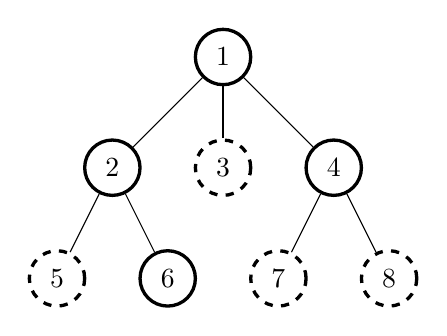
\begin{tikzpicture}[level distance=4em,sibling distance=4em,]
    
    \node (a1) [cir1] {1}
    child { node (a2)[cir1] {2}
        child { node (a5)[cir2] {5} } 
        child { node (a6)[cir1] {6} }
    }
    child { node (a3)[cir2] {3}}		
    child { node (a4)[cir1] {4}
        child { node [cir2] {7} } 
        child { node [cir2] {8} }
    };
    \end{tikzpicture}
    \caption{Sample graph with numbered node of two types}
    \label{fig:example-traversal1}
\end{figure}


%Another important notion that needs to be addressed is the comparison of graph nodes to each other and deciding whether two of them are the ``same'' in some sense or \textit{congruent}. 
%Latter in this chapter we will see that the important operations such as pattern matching depend on comparing nodes to derive whether they are ``the same''. 

%%%%
%% todo remove congruence; good congruence; good
%%%%
%Lets start with node comparison. The simplest form of equivalence, in the labelled graphs such as the one in Figure \ref{fig:example-traversal1}, is the equality of label values. In this example there are no two nodes that are the same because each of them have a unique label. But if we extend the notion of ``sameness'' from the equality of value to some other condition (or rule) then the mathematical term that captures this concept best is that of \textit{congruence} defined in Definition \ref{def:congreunce}. Lets take for example a simple arithmetic rule such as division by 2 which distinguishes odd and even nodes. Under this rule, two nodes are congruent if both are either even or both are odd. In Figure \ref{fig:example-traversal1} the nodes \{2, 4, 6, 8\} are congruent to each other because they are even and conversely the nodes \{1, 3, 5, 7\} are congruent as well. Another example of congruence rule is the node type distinction into continuous line circles and dashed line circles. Under this rule, in Figure \ref{fig:example-traversal1}, the nodes \{3, 5, 7, 8\} are congruent because they are dashed and the rest are congruent because they are in continuous line circles. 
%
%\begin{definition}[Congruence]\label{def:congreunce}
%    A \textit{congruence relation} (or congruence), denoted $\equiv$, is an equivalence relation on a structure that is compatible with the structure. Every congruence relation has a corresponding \textit{quotient} rule (or condition) forming an \textit{equivalence class} (or congruence class) for the relation \citep[26-27]{hungerford1980algebra}.
%\end{definition}
%
%In the case of sets or feature structures the congruence quotient rule needs to be defined corresponding to the structure. An example rule for set congruency can be the threshold of 2 elements on size of the set. Given three sets A=\{0, 1, 2\}, B=\{1, 2\}, C=\{5\}, D=\{6\}, under the above quotient rule, $A \equiv B$ and $C \equiv D$ forming the equivalence classes \{A, B\} and \{C, D\}. In Section \ref{sec:graph-matching} I will return to congruence relation between feature structures and will provide specific (quotient) rules that define equivalence between sets and feature structures. 

%%%%
%% end of congruence; good congruence; good
%%%%

%Lets turn now to queries over the graph nodes and edges. The notion of a query, defied in Definition \ref{def:query}, is tightly linked to the notion of congruence. The query is an operation that selects all the nodes or entities corresponding to a congruence class given by a quotient rule (or constraint) on a graph structure. For example in Figure \ref{fig:example-traversal1} a potential query is to return the equivalence class of the dashed nodes \{3, 5, 7, 8\}. The query operation can be extended to the the graph edges. 
%%In a given dependency graph, similar operation can be used to select all the determiner nodes. In that case we query the nodes with the condition that the part of speech has DT value i.e. \textit{pos=DT}. The same can be achieved by selecting all the edges connecting a noun to its determiner, then the query is formulated for all edges whose relation type is \textit{rel=det}.
%
%\begin{definition}[Graph query]\label{def:query}
%    %Given a graph $G=(V,E)$ to query nodes or edges is to select a set of nodes or a set of edges that satisfy the query constraint condition on feature structure.
%    Given a graph $G(V,E)$ and a query structure $F$, querying $q_{V}(F,G)$ or $q_{E}(F,G)$ over the nodes $V$ or edges $E$ of a graph $G$ is an operation that returns a set of nodes or edges equivalent to the query structure, $ \forall v \in V,  v \equiv F$. 
%\end{definition}

The \textit{graph traversal} defined in \ref{def:traversal} and especially its conditional and generative extensions defined in Definition \ref{def:conditional-traversal} and \ref{def:generative-traversal} are  important operations in this work. They are employed in the first phase of the algorithm, for copying the dependency graph as constituency graph described in Chapter \ref{ch:parsing-algorithm}. 

\begin{definition}[Traversal]\label{def:traversal}
    Traversal $t(V_S,G)$ of a graph $G$ starting from node $V_S$ is a recursive operation that returns a set of sequentially visited nodes neighbouring each other in either \textit{breadth first} ($t_{BF}$) or \textit{width first} ($t_{WF}$) orders.
\end{definition}

The graph traversal is employed either for searching for a node or an edge or finding a sub-graph that fulfils certain conditions on its nodes and edges if it is a conditional traversal. For example in the semantic enrichment phase (that will be described in Section \ref{sec:enrichment-stage}), to ensure that the semantic patterns are applied iteratively to each clause, from a multi-clause CG graphs are selected all clause sub-graphs without including the embedded (dependent) clauses. 

%Using sub-graphs for performing the pattern matching, like in the case of semantic enrichment, decreases drastically the complexity of the graph isomorphism problem (described in Section \ref{sec:graph-matching}) thus increasing the overall performance. 

\begin{definition}[Conditional Traversal]\label{def:conditional-traversal}
    Conditional traversal $t(F_V,F_E,V_S,G)$ of the graph $G$ starting from node $V_S$ under node conditions $F_V$ and edge conditions $F_E$ is a traversal operation where a node is visited if and only if its feature structure conditionally fulfils the $F_V$ and the edge that leads to this node conditionally fulfils the $F_E$.
\end{definition}

One of the potential complete traversals for the graph from Figure \ref{fig:example-traversal1} starting from the node 1 is \{1, 2, 3, 4, 5, 6, 7, 8\} using breadth first strategy or \{1, 2, 5, 6, 3, 4, 7, 8\} for depth first strategy. On the other hand, a conditional traversal of non-dashed nodes staring from the node 1 results in \{1, 2, 4, 6\}, \{1, 4, 2, 6\} or \{1, 2, 6, 4\}. The first two traversals corresponding to the width first strategy and the third one to the depth first strategy. 

I also use the graph traversal to execute generative operations on a parallel graph. For example DG traversal is employed for bootstrapping (i.e. creating in parallel) the CG as it was previously motivated in Section \ref{sec:architecture}.

\begin{definition}[Generative Traversal]\label{def:generative-traversal}
    Generative traversal $g(M,G)$ of a source graph $G$ via a operation matrix $M$ is an operation resulting in the creation of the target graph $H$ by contextually applying generative operations to bring the latter into existence. The operation matrix $M$ is a set of tuples $(ctx,o,p)$ that link the visited source node context $ctx$ (as features of the node, the edge and previously visited neighbour) to a certain operation $o$ that shall is executed on the target graph $H$ with parameters $p$.
\end{definition}

\tikzset{
    sqr1/.style={
        rectangle,
        draw=black, very thick,
        minimum height=0.5em,
        inner sep=0.5em,
        text centered,
        align=center,
        anchor=center
    }
}

\begin{figure}[!ht]
    \centering
    \begin{subfigure}[t]{0.28\textwidth}
        \centering
        \begin{tikzpicture}[scale=1]
        \node (a1) [cir1] { };
        \node (a11) [right =0.1em of a1] {= create};
        \node (a2) [cir2, below =2em of a1] { };
        \node (a21) [right =0.1em of a2] {= extend};
        \end{tikzpicture}
        \caption{The rule set}
        \label{fig:example-traversal00}
    \end{subfigure}
    \begin{subfigure}[t]{0.3\textwidth}
        \centering
        \begin{tikzpicture}[scale=1][level distance=4em,sibling distance=4em,]
        \node (a1) [sqr1] {a}
        child { node (a2)[sqr1] {b}
            child { node (a5)[sqr1] {d} } 
        }
        child { node (a3)[sqr1] {c}};
        \end{tikzpicture}
        \caption{The target}
        \label{fig:example-traversal21}
    \end{subfigure}
    \begin{subfigure}[t]{0.4\textwidth}
        \centering
        \begin{tikzpicture}[scale=1][level distance=4em,sibling distance=8em,]
        \node (a1) [sqr1] {a: \{1, 3\}}
        child { node (a2)[sqr1] {b: \{2, 5\}}
            child { node (a5)[sqr1] {d: \{6\}} } 
        }
        child { node (a3)[sqr1, right=1em of a2] {c: \{4, 7, 8\}}};
        \end{tikzpicture}
        \caption{The explained target}
        \label{fig:example-traversal22}
    \end{subfigure} 
    \caption{The generative traversal result for Figure \ref{fig:example-traversal1} using create and extend operations}
    \label{fig:example-traversal2}
\end{figure}

Next I provide an rough description of what happens when a generative traversal is executed and the exact algorithm will be described in detail in Section \ref{sec:creation-constituency-graph}. For example lets assume that only two types of operation are needed for our task at hand. First is to create a new node on the target graph once a non-dashed node is visited on the source graph. And, second, is to pass without doing anything the dashed nodes. This is schematically represented in Figure \ref{fig:example-traversal00}. Lets now apply these operations on traversing the example graph using breadth first strategy following the order provided above \{1, 2, 3, 4, 5, 6, 7, 8\}. The traversal graph is considered source graph and the target graph is empty at the beginning of the process. Upon visiting the node 1 a first node is created on the target graph which is labelled \textit{a}. When traversing nodes 2 and 4 then each of them signal creation of the nodes \textit{b} and \textit{c} as children of \textit{a} in the target graph and correspondingly node 6 signals creation of node \textit{d}. The final target graph is depicted in Figure \ref{fig:example-traversal21} and in Figure \ref{fig:example-traversal22} the source nodes are embedded into the target node to make explicit that the non-dashed nodes (i.e. 3, 5, 7, 8) are simply passed over without any generative operation. 

Now that generative traversal is defined, by analogy, \textit{update}, \textit{insert} and \textit{delete} traversals can be defined on the source or target graph by using the same mechanism of \textit{operation matrices} mapping contexts of visited nodes and edges to update, insert and delete operations. In this work, however, these operations are not used and therefore omitted here.

In Section \ref{sec:graphs} the last two definitions were for the constituency and dependency graphs. They are used in this thesis to represent grammatical analysis of of a sentence. Next we will look at a special type of graph which represents fragments of structure repeatable across multiple analysis. They represent generalisations or patterns that usually are associated with grammatical features or a set of features which I explain in Chapter \ref{ch:parsing-algorithm}. These graphs are called \textit{pattern graphs} and the next section is dedicated to them.  

\section{Pattern graphs}
\label{sec:pattern-graphs}
Regardless of the type, constituency or dependency, the parsing process (which will be described in Chapter \ref{ch:parsing-algorithm}) relies on identifying patterns in graphs. The patterning is described as both graph structure and feature presence (or absence) in the nodes or edges. The \textit{pattern graphs} (defined in \ref{def:graph-pattern}) are special kinds of graphs meant to represent small (repeatable) parts of parse graphs that, in the context of the current work, are used to identify grammatical features. 

The pattern graphs contrast with the \textit{parse} (or \textit{instance}) graphs which are either constituency or dependency graphs. The parse graphs express what is an actual analysis of a text, i.e. representing what is the case, whereas the pattern graph expresses a potential that could be the case in the instance graph. This way the pattern graphs have a prescriptive interpretation whereas the instance ones taken a factual interpretation. 

%Pattern graphs can also specify operations that shall be executed when the pattern is successfully matched (for example add a new feature on a given node). This kinds of graphs need last four requirements listed in the beginning of this section.

\begin{definition}[Pattern Graph]\label{def:graph-pattern}
    A \textit{pattern graph} (PG) is a feature rich graph for expressing regularities in the node and edge structure.
\end{definition}

%part of the definition: or edge configuration and feature structure including descriptions of \textit{negated nodes or edges} (i.e. absence of), logical operators over feature sets (AND, OR, XOR and NAND) and operations once the pattern is identified in a target graph (select, insert, delete and update).

%The feature structure of a PG are always \textit{underspecified} as compared to the dependency or constituency graph in the sense that irrelevant attribute-value pairs are omitted sometimes down to an empty FS. However often it is useful to specify more than one value for the same feature as a list of disjunctive values allowing the pattern to cover larger set of possible cases. I will call these FS as being \textit{over-specified}. 

%An example of PG is depicted in figure \ref{fig:gp1} in the Section \ref{sec:pattern-graph-matching}. It deals with pattern graph matching and other operations with in detail. But before that I will first briefly cover generic operations on graphs and the problem of graph matching also known in computer science as the \textit{graph isomorphism} problem.

%Before I dive into characterising pattern graph matching and operations with pattern graphs, I 
Next I discuss two example of pattern graphs. One example shows a pattern graph encoding the present perfect continuous tense, which traditional grammar defines as in Table \ref{tab:ppc-pattern}. Afterwards, the second example will show how the notion of linear succession among nodes is accounted for in the pattern graphs for declarative and interrogative mood.

\begin{table}[!ht]
	\centering
	\begin{tabular}{|clclc|}
		\hline
		\textit{has/have}       & + & \textit{been}          & + & \textit{Vb-ing}          \\
		to have, present simple &   & to be, past participle &   & verb, present participle \\ \hline
	\end{tabular}
	\caption{Present perfect continuous tense}
	\label{tab:ppc-pattern}
\end{table}

Examples \ref{ex:ppc1}--\ref{ex:ppc3} show variations of present perfect continuous tense in a simple clause according to declarative and interrogative mood and the ``has'' contraction. Of course there are more variations possible for example according to voice (active and passive) but they are omitted here because they adds combinatorially to the number of examples and the ones provided already serve their purpose here. The Figures \ref{fig:ppc1}-\ref{fig:ppc3} represent corresponding dependency parses for these examples (generated with Stanford dependency parser).

\begin{exe}
	\ex\label{ex:ppc1} He has been reading a text.
	\ex\label{ex:ppc2} He's been reading a text.
	\ex\label{ex:ppc3} Has he been reading a text?
\end{exe}

%\begin{figure}[!ht]
%	\centering
	\begin{figure}[!ht]
		\centering
		\begin{dependency}[dep-style-narrow]
			\begin{deptext}[]
				PRP \& VBZ \& VBN \& VBG \& DT \& NN \\
				He \& has \& been \& reading \& a \& text \\
			\end{deptext}
			\deproot{4}{root}
			\depedge{4}{1}{nsubj}
			\depedge{4}{2}{aux}
			\depedge{4}{3}{aux}
			\depedge{4}{6}{dobj}
			\depedge{6}{5}{det}
		\end{dependency}
		\caption{Present perfect continuous: indicative mood, un-contracted ``has''}
		\label{fig:ppc1}
	\end{figure}

	\begin{figure}[!ht]
        \centering
		\begin{dependency}[dep-style-narrow]
			\begin{deptext}[]
				PRP \& VBZ \& VBN \& VBG \& DT \& NN \\
				He \& 's \& been \& reading \& a \& text \\
			\end{deptext}
			\deproot{4}{root}
			\depedge{4}{1}{nsubj}
			\depedge{4}{2}{aux}
			\depedge{4}{3}{aux}
			\depedge{4}{6}{dobj}
			\depedge{6}{5}{det}
		\end{dependency}
		\caption{Present perfect continuous: indicative mood, contracted ``has'' }
		\label{fig:ppc2}
	\end{figure}
%\end{figure}
%
\begin{figure}[!ht]
	\centering
	\begin{dependency}[dep-style]
		\begin{deptext}[]
			VBZ \& PRP \& VBN \& VBG \& DT \& NN \\
			Has \& he \& been \& reading \& a \& text \\
		\end{deptext}
		\deproot{4}{root}
		\depedge{4}{2}{nsubj}
		\depedge{4}{1}{aux}
		\depedge{4}{3}{aux}
		\depedge{4}{6}{dobj}
		\depedge{6}{5}{det}
		%\depedge[collage]{5}{6}{dobj}
	\end{dependency}
	\caption{Present perfect continuous: interrogative mood, un-contracted ``has''}
	\label{fig:ppc3}
\end{figure}


The present perfect continuous tense can be formulated as a pattern graph (including voice) over the dependency structure as illustrated in Figure \ref{fig:gp1}.
In this pattern the main lexical verb is \textit{present participle} indicated via the \textit{VBG} part of speech. It is accompanied by two auxiliary verbs: \textit{to be} in \textit{past participle} (\textit{VBN}) form and \textit{to have} in \textit{present simple} form specified by either \textit{VBZ} for 3rd person or \textit{VBP} for non-3rd person. Also the \textit{to be} can be either connected by the \textit{aux} relation or in case of passive form by the \textit{auxpass} relation. Note that the pattern in Figure \ref{fig:gp1} constraints the edge type (using an OR-set) to the verb \textit{to be} which can be either \textit{aux} or \textit{auxpass} and the part of speech of the verb \textit{to have} which can be \textit{VBZ} or \textit{VBP}.

\begin{figure}[!ht]
    \centering
    \begin{tikzpicture}[tree-style]
    \node[pattern-node, anchor=center] (vb1){pos:VBG}
    child {node[pattern-node] {lemma:be\\pos:VBN} edge from parent node[left] {rel:$_{OR}$[aux,auxpass]} }
    child {node[pattern-node] {lemma:have\\pos:$_{OR}$[VBZ,VBP]} edge from parent node[right] {rel:aux}};
    \end{tikzpicture}
    \caption{The graph pattern capturing features of the present perfect continuous tense}
    \label{fig:gp1}
\end{figure}

One of the fundamental features of language is its sequentiality and directionality. This aspect is not inherent in graphs. In the simplest form, they just describe connections between nodes and are agnostic to any meaning or interpretation. Next, I introduce the way I deal with linear order in the pattern graphs. 

%To demonstrate how the order will specified in the graph patterns, 
Lets consider the clause mood and encode the distinction between \textit{declarative} and \textit{Yes/No interrogative} moods. In SFG this features is described in terms of the relative order of clause elements. If the finite is before the subject then the mood is Yes/No-interrogative, whereas when the finite succeeds subject then the mood is declarative. Example \ref{ex:ppc3} contrasts in mood with \ref{ex:ppc1} and \ref{ex:ppc2}. 

Order can be specified in absolute or relative terms and partially or exhaustively. In order to cover these three kinds of constraints, I introduce three special features: the node \textit{id}, \textit{precede} and \textit{position}. Node id takes a token to uniquely identify a node in the graph, the precede feature takes an ordered set to indicate the (partial) linear precedence to other node ids, and the position feature indicates the absolute position of a node.

One way to introduce order among nodes is then by marking them with an absolute position. This is a good method applicable to parse graphs. The DGs and CGs, are automatically assigned at creation time the absolute position of the node in the sentence text via the feature \textit{position}. This feature is present in the leaf nodes only and corresponds to the order number in which they occur in the sentence text while the non-leaf node's position is considered to be the lowest position of its constituent nodes. The absolute position description is rarely used in the PGs. The only cases are to state that the constituent is first or last position in a sentence.  %In the 

Another way to specify node order is through relative precedence, for which the node id and the precedence features are introduced above. This is the preferred method to provide linear precedence dimension in pattern graphs. It is also relative so the specification can be partial. With this method a node specifies that it precedes a set of other nodes. 

	\begin{figure}[!ht]%{0.4\textwidth}
		\centering
		\begin{tikzpicture}[tree-style,]
		\node (cla) [pattern-node] {class:clause}
		child { node (sub)[pattern-node] {element:subject,\\position:1}}		
		child { node (f)[pattern-node] {element:finite,\\position:2}};
		\end{tikzpicture}
		\caption{Declarative mood pattern graph with relative element order}
		\label{fig:pg-declarative}
	\end{figure}
	\begin{figure}[!ht]%{0.4\textwidth}
		\centering
		\begin{tikzpicture}[tree-style,]
		\node (cla) [pattern-node] {class:clause}
		child { node (sub)[pattern-node] {element:subject,\\id:s1, precede:f1}}		
		child { node (f)[pattern-node] {element:finite,\\id:f1}};
		\end{tikzpicture}
		\caption{Declarative mood pattern graph with absolute element order}
		\label{fig:pg-declarative2}
	\end{figure}
    \begin{figure}[!ht]
    	\centering
    	\begin{tikzpicture}[tree-style,]
    	\node (cla) [pattern-node] {class:clause}
    	child { node (f)[pattern-node] {element:finite,\\id:f1, precede:s1}}
    	child { node (sub)[pattern-node] {element:subject,\\id:s1}}	;	
    %	child { node (mv)[pattern-node] {element:main verb,\\id:mv1}};
    	\end{tikzpicture}
    	\caption{Pattern graph for Yes/No interrogative mood}
    	\label{fig:pg-interrogative}
    \end{figure}

To continue the example of mood features, I illustrate in Figures \ref{fig:pg-declarative} and \ref{fig:pg-declarative2} the use of relative and absolute node ordering constraints for declarative mood; and in 
Figure \ref{fig:pg-interrogative}, I depict the PG for the Yes/No interrogative mood. In both cases I use the relative node ordering.

%todo: explain what negative nodes are

%From the usability point of view there are few technicalities I shall emphasize. First, the precedence feature can be used on any node. When matched, the precedence declarations are collected from all nodes into a single set before being checked. However I recommend as a good practice to specify the order of nodes on the parent constituent. 
%
%Second, the notation in Figure \ref{fig:pg-interrogative} follows the Python bracketing meaning i.e. the round brakes signify tuples while the square ones lists (ordered sets). So the main verb element is redundant and is introduced to demonstrate multiple order specifications. However the order can be either specified as a set of binary tuples or as an ordered set (i.e. a Python list). So precedence:[(f1,s1),(s1,mv1)] is equivalent to precedence:[f1,s1,mv1]. 
%
%Thirdly the ordering can be defined in absolute terms via position or in relative terms. Note that in the case of PGs the absolute ordering of nodes is interpreted relatively so PG in figure \ref{fig:pg-declarative} is identical to \ref{fig:pg-declarative2}.


Patterns like the ones explained above can be created for a wide range of grammatical features. Once the grammatical feature is encoded as a pattern graph it can be identified in parse graphs (DG or CG) via \textit{graph pattern matching} operation described in Section \ref{sec:graph-matching}. Moreover, once the pattern is identified it can act as a triggering condition to for various operation. For example an operation can be to inject the identified feature into the parse graph and this way enriching its content. Coming back to out tense example above, once the pattern \ref{fig:gp1} is identified then the clause can be marked with the tense feature. In the next section I address in detail the graph matching operation and then show how it works using pattern graphs. 

% skip:complicated, unclear, compressed
%But such traversal operations cannot be easily defined. While traversal context may be sufficient for generative operations on a new structure, it is insufficient for executing affecting operations on the traversed graph. To overcome this limitation, instead of using traversal context I take a different approach: the \textit{pattern graphs}, defined in previous section combined with generic graph matching algorithm. This mechanism offers a similar algorithmic independence of mapping structural context to operation(s) triggered by it. 

\section{Graph matching}
\label{sec:graph-matching}

So far we have discussed about constituency and dependency graphs and, in the last section, I introduced pattern graphs. The intuition behind pattern graphs is that they are meant to be matched against or found in other (instance) graphs. I will address now what does it mean for two graphs to be the same, i.e. \textit{(structurally) isomorphic}, and what does it mean in the current work. In mathematics the structure-preserving mappings from one structure to another one of the same type is called \textit{morphism}. 

\begin{definition}[Morphism]\label{def:morphism}
    A morphism $f:X \rightarrow Y$ is a structure preserving map from one object $X$ to the other $Y$ where the objects are complex structures such as sets, feature structures or graphs.
\end{definition}


\begin{definition}[Isomorphism]\label{def:isomorphism}
    The morphism $f:X \rightarrow Y$ is called \textit{isomorphism} if there exists an inverse morphism $g:Y \rightarrow X$ such that $f \circ g = id_{X}$ and $ g \circ f = id_{X}$.
\end{definition}

The graph matching is known in computer science as (sub-)graph isomorphism testing. Two graphs $G=(V_G,E_G)$ and $H=(V_H,E_H)$ are isomorphic if mapping the nodes of $G$ with the nodes of $H$, preserving the edge neighbourhood, results in graph $H$. 
%The operation of testing the graph isomorphism is called graph matching. 

\begin{definition}[Graph matching]\label{def:gmatching}
    For two graphs $G$ and $H$, where $G \leq H$, \textit{graph matching} is the operation of finding an isomorphism between $G$ and $H$.
\end{definition}

\begin{definition}[Graph isomorphism]\label{def:gisomorphism}
    An isomorphism of graph $G=(V_G,E_G)$ and $H=(V_H,E_H)$ is a bijective function $f:V_G \rightarrow V_H$ such that if any two nodes  $u,v \in V_G$ from $G$ are adjacent $(u,v) \in E_G$ then $f(u), f(v)$ are adjacent in $H$ as well $(f(u), f(v)) \in E_H $.
\end{definition}

%\begin{definition}[Graph matching]\label{def:gmatching0}
%    For two given graphs $G$ and $H$ \textit{graph matching} is the operation of testing whether $G$ is structurally isomorphic to $H$.
%\end{definition}

Graphs do not need to have the same number of nodes or edges. We say that a graph is smaller than another one, denoted $G \leq H$, when its number of nodes is less than that of the other graph. In this case the isomorphism is established to a sub-graph of $H$. 
The pattern graphs, employed in the current work, are usually simpler and smaller than the (constituency or dependency) graph they are matched against. 
%In such cases the task is to identify whether the first, smaller graph, is isomorphic to a sub-graph of the second one. 
In this case, the mapping function is relaxed from bijective (perfect mapping from first to second graph) to an injective one (each node from first has a correspondent in the second one).

\begin{definition}[Sub-graph isomorphism]\label{def:sgisomorphism}
       Given two feature rich graphs $G=(V_G,E_G)$ and $H=(V_H,E_H)$, $G$ is sub-graph isomorphic to $G$ (denoted $G \subseteq H$) if there is an injective function $f:V_G \rightarrow V_H$ such that
   \begin{itemize}
       \item $\forall v \in V_G, f(v) \in V_H$ and
       \item any two nodes adjacent in $G$, $(u,v) \in E_G$, are also adjacent in $H$, $(f(u), f(v)) \in E_H $
   \end{itemize}
\end{definition}


\begin{figure}[!ht]
    \centering
    \begin{subfigure}[t]{0.48\textwidth}
        \centering
        \begin{tikzpicture}[scale=1]
        \node (a1) [cir1] {1};
        \node (a2) [cir1, right =3em of a1] {2};
        \node (a3) [cir1, below =3em of a1] {3};
        
         \draw[sequence,->] (a1) -- (a2);
         \draw[sequence,->] (a2) -- (a3);
         \draw[sequence,->] (a3) -- (a1);
        
        \end{tikzpicture}
        \caption{The pattern graph}
        \label{fig:example-matching1}
    \end{subfigure}
    \begin{subfigure}[t]{0.48\textwidth}
        \centering
        \begin{tikzpicture}[scale=1][level distance=4em, sibling distance=4em,]
        \node (a1) [cir1] {a};
        \node (a2) [cir1, right =3em of a1] {b};
        \node (a3) [cir1, below =3em of a1] {c};
        \node (a4) [cir1, below =3em of a2] {d};
        
        \draw[sequence,->] (a1) -- (a2);
        \draw[sequence,->] (a2) -- (a3);
        \draw[sequence,->] (a3) -- (a1);
        \draw[sequence,->] (a2) -- (a4);
        
        \end{tikzpicture}
        \caption{The target graph}
        \label{fig:example-matching2}
    \end{subfigure}
    \caption{Sub-graph isomorphism \{1=a, 2=b, 3=c\}}
    \label{fig:example-matching}
\end{figure}

In Figure \ref{fig:example-matching1} is depicted a labelled graph that is isomorphic to a sub-graph in Figure \ref{fig:example-matching2}. The example graphs presented in Figure \ref{fig:example-matching} have atomic labels as nodes and the isomorphism is established as a mapping between labels. Section \ref{sec:graphs} above mentions that the graph considered in this thesis have feature structures as their nodes and not atomic nodes. But in case of feature rich graphs additional rules how to establish the isomorphism need to be provided because there are multiple ways to approaching it. 

\begin{figure}[!ht]
    \centering
    \begin{subfigure}[t]{0.38\textwidth}
        \centering
        \begin{tikzpicture}[scale=1]
        \node (a1) [pattern-node] {f_1: 1 \\ f_2: scissors};
        \node (a2) [pattern-node, right =3em of a1] {f_1: 2 \\ f_2: paper};
        \node (a3) [pattern-node, below =3em of a1] {f_1: 3 \\ f_2: rock};
        
        \draw[sequence,->] (a1) -- (a2);
        \draw[sequence,->] (a2) -- (a3);
        \draw[sequence,->] (a3) -- (a1);
        
        \end{tikzpicture}
        \caption{The pattern graph}
        \label{fig:example-r-matching1}
    \end{subfigure}
    \begin{subfigure}[t]{0.58\textwidth}
        \centering
        \begin{tikzpicture}[scale=1][level distance=4em, sibling distance=4em,]
        \node (a1) [pattern-node] {f_1: a \\ f_2: scissors};
        \node (a2) [pattern-node, right =3em of a1] {f_1: b \\ f_2: paper};
        \node (a3) [pattern-node, below =3em of a1] {f_1: c \\ f_2: rock};
        \node (a4) [pattern-node, below =3em of a2] {f_1: d \\ f_2: scissors};
        \node (a5) [pattern-node, right =3em of a4] {f_1: e \\ f_2: rock};
        
        \draw[sequence,->] (a1) -- (a2);
        \draw[sequence,->] (a2) -- (a3);
        \draw[sequence,->] (a3) -- (a1);

        \draw[sequence,->] (a2) -- (a4);
        \draw[sequence,->] (a4) -- (a5);
        \draw[sequence,->] (a5) -- (a2);
        
        \end{tikzpicture}
        \caption{The target graph}
        \label{fig:example-r-matching2}
    \end{subfigure}
    \caption{An example of rich sub-graph isomorphism}
    \label{fig:example-r-matching}
\end{figure}

Lets look at Figure \ref{fig:example-r-matching} where the graph nodes are feature structures using features: f_1 and f_2. One way to approach isomorphism in this scenario is by the value of one feature, for example f_1. Then we can identify two sub-graph isomorphisms: \{1=a, 2=b, 3=c\} and \{1=b, 2=d, 3=e\}. This approach, besides additional specification what values to compare, i.e. f_1s, is the same as providing a sub-graph isomorphism on the labelled graphs from Figure \ref{fig:example-matching}. 

In addition to the rule above, lets add a constraint that the isomorphism is not only a mapping between the feature values (numbers to letters) but also that the mapped values are identical (strict value equality). 
If we consider the strict equality rule applied on f_1 feature, there is no isomorphism between the two graphs because first one uses numbers  \{1, 2, 3\} and the second uses letters\{a, b, c, d\}. Now if we turn to the values of f_2 and apply the same rule then there is one isomorphism possible \{paper=paper, rock=rock, scissors=scissors\}. The second one, even if it is a cycle, \{paper=paper, rock=scissors, scissors=rock\} is no longer acceptable because the ``scissors'' and ``rock'' switched places in the target graph and it would have been acceptable as a mapping, but not as strict value equality. Formally, the additional equality constraint can be expressed on the graph isomorphism $f$ as $u=f(u)$.

This brings us to the idea that, in the feature rich (sub-)graph isomorphism, a \textit{matching} relation (denoted $\match$)for nodes needs to be considered. And as the FS constitute the graph nodes then the matching relations needs to be defined on the FS. We say that a feature structure may match once, several times or not at all another feature structure, $FS_1 \match FS_2$. This intuition is expressed in Definition \ref{def:fs-match}.
The FS matching is in accordance with the goals of the particular task or satisfying a certain set of conditions. Thus replacing the label equality with matching criteria is the method to impose an additional set of constraints on the graph isomorphism and allow comparison of complex nodes such as those in feature rich graphs. This is expressed in Definition \ref{def:rsgisomorphism} below. 
%The rich graph matching operation can be also seen as a search for rich sub-graph isomorphism. 

\begin{definition}[Rich sub-graph isomorphism]\label{def:rsgisomorphism}
    Given two feature rich graphs $G=(V_G,E_G)$ and $H=(V_H,E_H)$ and a matching relation $\match$, $G$ is sub-graph isomorphic to $H$ if there is an injective mapping $f:V_G \rightarrow V_H$ such that
    \begin{itemize}
        \item each node in $V$ is mapped to exactly one node in $H$, $\forall v \in V_G, f(v) \in V_H$ and
        \item each node in $G$ matches with its correspondent in $H$, $\forall v \in V_G, v \gtrdot f(v)$ and
        \item any two nodes which are adjacent in $G$, are also adjacent in $H$, $\forall (u,v) \in E_G, \exists \big(f(u), f(v)\big) \in E_H $
    \end{itemize}
\end{definition}

%\begin{definition}[Rich Graph Matching]\label{def:rgmatching}
%    For two feature rich graphs $G$ and $H$ where $H \leq G$ and an \textit{identity settling function} $idx_{V}$, the \textit{rich graph matching} is the function that finds a structural isomorphism between $H$ and $G_{1} \subseteq G$ provided that for all nodes $V_{i} \in H$ their \textit{morphism function} $V_{j} \in G_{1}$ 
%    
%    satisfies the identity function $f_{V}(V_{i})=V_{j}$ 
%\end{definition}

%The congruency rules (also referred in the implementation as \textit{identity} or \textit{equivalence functions}) used in this work will be provided in the Section \ref{sec:pattern-graph-matching} below. They are contextualised to the graph matching operation between pattern graphs and dependency and constituency graphs. 
%
%\section{Pattern graph matching}
%\label{sec:pattern-graph-matching}

A particular case of graph matching, of important to the current work, is the \textit{pattern graph matching} (Definition \ref{def:pgmatching}) which is an operation to identify patterns in the dependency or constituency  \textit{parse graphs} following the \textit{strict feature matching} on their nodes defined in Definition \ref{def:fs-match} below. 

\begin{definition}[Pattern graph matching]\label{def:pgmatching}
    Given a pattern graph $G$ and an instance (parse) graph $H$ (either dependency or constituency), \textit{pattern graph matching} is the operation of finding a rich sub-graph isomorphism from $G$ to $H$ such that each pattern node matches its corresponded instance node each $H$, $\forall v \in V_G, v \gtrdot f(v)$. 
\end{definition}

%The pattern and parse graphs are feature rich graphs. This means that the nodes are feature structures. In the previous section the rich graph matching require definition of congruence rules and in this case it is between two feature structures. 

As mentioned before, nodes of the parse and the pattern graphs are feature structures. I approach the matching between them in two steps: first, matching the feature names in Definition \ref{def:fs-match}, and second,  matching the feature values in Table \ref{tab:strict}. 
In order to simplify and make explanations clear, I will further refer to the feature structures that constitute nodes in the pattern graphs as \textit{pattern feature structures} and the feature structures that constitute nodes in the instance graphs as \textit{instance feature structure}.

\begin{definition}[Feature structure matching]\label{def:fs-match}
    A pattern feature structure $V$ matches an instance feature structure $U$ if and only if every feature in $V$ has a corresponding feature $U$ and their values match; that is $ \forall f_V \in V, \exists f_U$ such that $name(f_V) = name(f_U)$ and $ val(f_V) \match val(f_U)$.
\end{definition}

Next is defined matching of the feature values. According to the Definition \ref{def:fs}, the values of feature structures can be either atomic (numbers, strings, symbols, etc.), denoted $atomic$, or one of the conjunction sets: $S_{AND}$, $S_{OR}$, $S_{XOR}$ and $S_{NAND}$. For simplicity, the option of nested feature structures is excluded in the current work even though it is perfectly viable configuration. Consequently, the matching relation takes into consideration the \textit{type} of the compared elements in addition to how they relate to each other, including comparisons between set and atomic values. 
Furthermore this relation is \textit{not symmetric} or \textit{not commutative} because the subsequent relations used in the definition are not symmetric (e.g. set inclusion or set subsumption). 
This means that we cannot switch places of the compared elements or if we do then they will yield different results, $A \match B \neq B \match A $. 
%Finally, these definitions create equivalence sets \textit{relative} to one of the compared elements and not absolute equivalence sets. For example the division by 2, is an absolute condition for two numeric elements to belong to the same equivalence class either of odd or that of even numbers. By contrast, if we consider set inclusion between two sets $A \subseteq B$ as a condition for set element equivalence then it generates two possible equivalence sets. First, all sets $X$ that are subsets of $B$, $\forall X, X \subseteq B$ and second, all sets Y that include $A$,  $ \forall Y, A \subseteq Y $. 

The function $\tau(S)$, defined in Section \ref{sec:graphs}, which returns the type of the feature value is extended here to handle also atomic data types in addition to sets and is defined as follows $\tau:x \rightarrow \{atomic, S_{AND}, S_{OR}, S_{XOR}, S_{NAND} \}$. The matching rules have to be defined for each possible pair of types returned by the function $\tau$ yielding 25 possibilities. Table \ref{tab:strict} provides matching relations for each pair of types. Each cell contains a boolean or comparison expression returning a truth value where the rows represent value types of the pattern features, denoted $\tau(v)$, and the columns represent value types of the instance features, denoted $\tau(u)$. Cells with a bottom sign $\bot$ mean that there can be no match between these types no matter the values. 
%I use set theoretic notations such as set inclusion $\subseteq$, intersection $\cup$ and set membership $\in$. 

\begin{table}[!ht]
    \centering
    \begin{tabular}{|c|c|c|c|c|c|}
        \hline
        \textit{$\tau(v)$\textbackslash $\tau(u)$} & \textit{atomic} & \textit{S_{AND}}                 & \textit{S_{OR}}              & \textit{S_{XOR}}             & \textit{S_{NAND}}            \\ \hline
        \textit{atomic}             & $v=u$             & $v \in u$                         & $\bot$                          & $\bot$                          & $v \notin u$                   \\ \hline
        \textit{S_{AND}}              & $\bot$               & $v \subseteq u$                     & $\bot$                          & $\bot$                          & $\bot$ \\ \hline
        \textit{S_{OR}}               & $v \ni u$          & $ v \cap u \neq \varnothing $ &                        $v \supseteq u $              & $v \supseteq u $   & $\bot$ \\ \hline
        \textit{S_{XOR}}              & $v \ni u$          & $\bot$                              & $\bot$                        & $v \supseteq u$             & $\bot$ \\ \hline
        \textit{S_{NAND}}             & $v \not\ni u$      & $v \cap u = \varnothing$     & $v \cap u = \varnothing$ & $v \cap u = \varnothing$ & $ v \subseteq u $                          \\ \hline
    \end{tabular}
    \caption{Strict matching between pattern and instance feature values organised by value type}
    \label{tab:strict}
\end{table}

For example, if both values are of atomic type then in order to match they have to equal. If the $\tau(v)$ is atomic and the $\tau(u)$ is an AND set then $v$ needs to be among the set of values constituting $u$; whereas if the $\tau(u)$ is an OR or XOR set then these values do not match, designated by the bottom sign $\bot$. The same reading applies to the rest of the table for each pair of value types. 

A more permissive matching is defined in Table \ref{tab:permissive}. Here, on the instance feature values, the two types of disjunction (OR and XOR) and the negated conjunction (NAND) are interpreted as possibly matching and provided with the corresponding relation whereas in the previous definition these cases were completely excluded. The permissive match is rarely used in this work but it is nevertheless useful cases of instance graphs where the feature values could not be are assigned with a certainty but as a disjunction of either one or the other. 

\begin{table}[!ht]
    \centering
    \begin{tabular}{|c|c|c|c|c|c|}
        \hline
        \textit{$\tau(v)$\textbackslash $\tau(u)$} & \textit{atomic} & \textit{S_{AND}}                 & \textit{S_{OR}}              & \textit{S_{XOR}}             & \textit{S_{NAND}}            \\ \hline
        \textit{atomic}             & $v=u$             & $v \in u$                         & $v \in u$                          & $v \in u$                          & $v \notin u$                   \\ \hline
        \textit{S_{AND}}              & $\bot$               & $v \subseteq u$                     & $v \subseteq u$                          & $v \subseteq u$                          & $v \cap u = \varnothing$ \\ \hline
        \textit{S_{OR}}               & $v \ni u$          & $ v \cap u \neq \varnothing $ &                        $v \supseteq u $              & $v \supseteq u $   & $v \backslash u \neq \varnothing$ \\ \hline
        \textit{S_{XOR}}              & $v \ni u$          & $\bot$                              & $\bot$                        & $v \supseteq u$             & $ |v \backslash u| = 1$ \\ \hline
        \textit{S_{NAND}}             & $v \not\ni u$      & $v \cap u = \varnothing$     & $v \cap u = \varnothing$ & $v \cap u = \varnothing$ & $ v \subseteq u $                          \\ \hline
    \end{tabular}
    \caption{Permissive matching between pattern and instance feature values organised by value type}
    \label{tab:permissive}
\end{table}


%the old taxt no longer needed
%
%
%When checking the equivalence of two feature values, three cases can be asserted: $x=y$ i.e. $x$ is definitely equal to $y$, $x\neq y$ i.e. $x$ is definitely different from $y$ and $x\sim y$ i.e. $x$ is maybe (or could be) equal to $y$. 
%
%I define below two identity morphisms: (a) \textit{permissive} $I_{permissive}$ (defined by Equation \ref{eq:permissive}) which includes the uncertain cases and (b) \textit{strict} $I_{strict}$ (defined by Equation \ref{eq:strict}) which excludes the uncertain cases. The main difference between the two morphism functions is whether on the right side (the instance graph) any uncertainty is accepted. This is to say any of the disjunctive sets $s_{OR}$ and $S_{XOR}$. 
%
%\begin{definition}[Strict Pattern Graph Matching]\label{def:strict-matching}
%	\textit{Strict pattern graph matching} is a rich graph matching where a morphism for the pattern graph $H$ is found in the target graph $G$ given that $H \leq G$ and that for any node $p \in H$ there is a node $r \in G$ satisfying the strict identity morphism $I_{strict}:p \rightarrow r$
%\end{definition}
%
%
%\begin{equation} \label{eq:strict}
%	I_{strict}:p \rightarrow r \models
%	\begin{cases}
%	p = r, & \text{if}\ T(p) = simple \wedge T(r) = simple \\
%	p \in r, & \text{if}\ T(p) = simple \wedge T(r) = S_{AND} \\
%	p \subseteq r, & \text{if}\ T(p) = S_{AND} \wedge T(r)= S_{AND} \\
%	p \cap r \neq \varnothing, & \text{if}\ T(p) = S_{OR} \wedge T(r) = S_{AND}\\
%	r \in p, & \text{if}\ T(p) = S_{OR} \wedge T(r) = simple \\
%	%p \cap r \neq \varnothing, & \text{if}\ T(p) = S_{XOR} \wedge T(r) \in \{S_{OR}, S_{XOR}\} \\
%	r \in p, & \text{if}\ T(p) = S_{XOR} \wedge T(r) = simple \\
%	p \cap r = \varnothing, & \text{if}\ T(p) = S_{NAND} \wedge T(r) \in \{S_{AND}, S_{OR}, S_{XOR}\} \\
%	r \notin p, & \text{if}\ T(p) = S_{NAND} \wedge T(r) = simple \\
%	\top, & \text{if}\ T(p) = S_{NAND} \wedge T(r) = S_{NAND}
%	\end{cases}
%\end{equation}
%
%\begin{definition}[Permissive Pattern Graph Matching]\label{def:permissive-matching}
%	\textit{Permissive pattern graph matching} is a rich graph matching where a morphism for the pattern graph $H$ is found in the target graph $G$ given that $H \leq G$ and that for any node $p \in H$ there is a node $r \in G$ satisfying the permissive identity morphism $I_{permissive}:p \rightarrow r$
%\end{definition}
%
%\begin{equation} \label{eq:permissive}
%	I_{permissive}:p \rightarrow r \models
%	\begin{cases}
%	p = r, & \text{if}\ T(p) = simple \wedge T(r) = simple \\
%	p \in r, & \text{if}\ T(p) = simple \wedge T(r) \in \{S_{AND}, S_{OR}, S_{XOR}\} \\
%	p \subseteq r, & \text{if}\ T(p) = S_{AND} \wedge T(r) = S_{AND} \\
%	p \cap r \neq \varnothing, & \text{if}\ T(p) = S_{OR} \wedge T(r) \in \{S_{AND}, S_{OR}, S_{XOR}\}\\
%	r \in p, & \text{if}\ T(p) = S_{OR} \wedge T(r) = simple \\
%	p \cap r \neq \varnothing, & \text{if}\ T(p) = S_{XOR} \wedge T(r) \in \{S_{OR}, S_{XOR}\} \\
%	r \in p, & \text{if}\ T(p) = S_{XOR} \wedge T(r) = simple \\
%	p \cap r = \varnothing, & \text{if}\ T(p) = S_{NAND} \wedge T(r) \in \{S_{AND}, S_{OR}, S_{XOR}\} \\
%	r \notin p, & \text{if}\ T(p) = S_{NAND} \wedge T(r) = simple \\
%	\top, & \text{if}\ T(p) = S_{NAND} \wedge T(r) = S_{NAND}
%	\end{cases}
%\end{equation}

Of course the matching rules proposed in Definition \ref{def:fs-match} and Table \ref{tab:strict} are not the only one that can be defined for the pattern matching. 
%A more permissive forms are possible, for example checking subset set inclusion for OR and XOR sets which currently is excluded.   
To handle this possible variation, in the parser implementation, the pattern matching function takes as parameter the matching relation, i.e. the identity function. The only constraints, on such a function, are to return a truth value and to take two parameters. The implementation also supports identity function for edges as well. In this work, all the pattern matching is performed entirely on constituent graphs (whose edges have no labels) and none on the dependency graphs (whose edges have labels), therefore I skip entirely the discussion about the edge matching in a sub-graph isomorphism. Nonetheless, the matching definitions above apply to matching edge features feature values too. 

Now that pattern graph matching is explained, lets take a look next at how it is used to perform operation on instance graphs.

\section{Pattern based operations}
\label{sec:pattern-based-operations}

The patterns are searched for in a graph always for a purpose. Graph isomorphism is only a precondition for another operation, be it a simple selection (i.e. non-affecting operation) or an affecting operation such as feature structure enrichment (on either nodes or edges), inserting or deleting a node or drawing a new connection between nodes. It seems only natural that the end goal is embedded into the pattern, so that when it is identified, also the desired operation(s) is(are) triggered. I call such graph patterns \textit{operational pattern graphs} (Definition \ref{def:operational-pattern}). Next I explain how to embed the operations into the graph pattern and how they are used in the algorithm. 

\begin{definition}[Operational graph pattern]\label{def:operational-pattern}
    An \textit{operative graph pattern} is a pattern graph that has least on one node \textit{operation} and \textit{arg} features.
\end{definition}

The operational aspect of the pattern graph is specified in the node FS via three special features: \textit{id}, \textit{operation} and \textit{arg}. The \textit{id} feature (the same as for relative node ordering) is used to mark the node for further referencing as an argument of an operation, the \textit{operation} feature names the function to be executed once the pattern is identified and the \textit{arg} feature specifies the function arguments if any required and they are tightly coupled with function implementation. If a node has the feature operation then it is called \textit{operational node}. Also, in the current implementation, the special features such as operation, arg, id, precede etc. are excluded from the pattern matching operation because they have functional role linked to the implementation and do not describe the linguistic properties of a graph node.

So far the implemented operations are \textit{insert}, which is used for creation of empty nodes, \textit{delete}, which is used for corrections of predictable errors in dependency graphs and \textit{update} operation, which is the main mechanism behind graph enrichment. These operations are depicted in Figure \ref{fig:pipeline-overview} of the parser pipeline architecture from Section \ref{sec:architecture}.

Operative patterns are enacted once they are matched to an instance graph. 
An operative pattern graph $G$ is \textit{enacted} on an instance graph $H$, in two steps. First, the pattern graph is strictly matched to instance graph. If an isomorphism $f$ is found then, second, for every operational node $v \in G, \exists att(v)=operation$, the specified operation $op = val(v.operation)$ and the corresponding node of the instance graph $u \in H$, the operation is executed on the node of the instance graph $op(u)$. If the arg feature is provided then the operation is executed with that additional argument. 

\subsection{Pattern based node update} 

As mentioned above the pattern based node update is used for adding onto the constituency graph new features. Lets consider Example \ref{ex:transitivity1} whose constituency graph is provided in Figure \ref{fig:cg-transitive1} and the task to assign \textit{agent} feature to the subject node and \textit{affected-possessed} feature to the complement. This can be done using the pattern graph matching with a feature update operation indicated on subject and complement nodes. The PG depicted in Figure \ref{fig:pg-transitive1} fulfils this purpose because it matches constituency graph from Figure \ref{fig:cg-transitive1} and has the corresponding update operations indicated.

\begin{exe}
    \ex\label{ex:transitivity1} He gave the cake away.
    \ex\label{ex:transitivity2} He gave her the cake.
\end{exe}

%\begin{table}[!ht]
%    \centering
%    \begin{tabular}{|c|c|c|c|c|}
%        \hline
%        \multicolumn{5}{|c|}{clause}                                                               \\ \hline
%        subject & main verb & \multicolumn{2}{c|}{complement} & adjunct \\ \hline
%        He              & gave               & the               & cake               & away.            \\ \hline
%    \end{tabular}
%    \caption{CG with a transitive verb}
%    \label{tab:transitive1}
%\end{table}

%The constituency graph representation for the clause analysis from Table \ref{tab:transitive1} is depicted in Figure \ref{fig:cg-transitive1}. 

\begin{figure}[!ht]
    \centering
    \scalebox{0.7}{
    \begin{tikzpicture}[
    tree-style, 
%    edge-style,
    level 1/.style={sibling distance=10em},
    level 2/.style={sibling distance=8em},
    level distance = 4em
    ]
    \node[pattern-node]{class: clause}
    child {node[pattern-node]{element: subject\\word: He} }
    child {node[pattern-node]{element: main verb\\word: gave} }
    child {node[pattern-node]{element: complement\\class: nominal group}  {}
        child {node[pattern-node]{element: deictic\\word: the} }
        child {node[pattern-node]{element: thing\\word: cake} }
    }
    child {node[pattern-node]{element: adjunct\\word: away}  }
    ;
    \end{tikzpicture}
}
    \caption{Constituency graph corresponding to Example \ref{ex:transitivity1}}
    \label{fig:cg-transitive1}
\end{figure}
\begin{figure}[!ht]
\centering
\scalebox{0.7}{
\begin{tikzpicture}[tree-style, level 1/.style={sibling distance=14em}, level distance = 5em]
\node[pattern-node]{element:clause}
	child {node[pattern-node, xshift=1.5em]{element: subject\\operation: update\\arg1:\{participant: agent\}} }
   	child {node[pattern-node]{element: main verb\\word: give\\operation: update\\arg1:\{process: possessive\}} }
    child {node[pattern-node, xshift=1em]{element: complement\\operation: update\\arg1:\{participant: affected-possessed\}}};
\end{tikzpicture}
}
\caption{A graph pattern for inserting agent and affected-possessed participant roles}
\label{fig:pg-transitive1}
\end{figure}
\begin{figure}[!ht]
    \centering
    \scalebox{0.7}{
        \begin{tikzpicture}[
        tree-style, 
        %    edge-style,
        level 1/.style={sibling distance=12em},
        level 2/.style={sibling distance=8em},
        level distance = 5em
        ]
        \node[pattern-node]{class: clause}
        child {node[pattern-node, xshift=2em]{element: subject\\\textit{participant: agent}\\word: He} }
        child {node[pattern-node]{element: main verb\\\textit{process: possessive}\\word: gave} }
        child {node[pattern-node]{element: complement\\\textit{participant: affected-possessed}\\class: nominal group}  {}
            child {node[pattern-node]{element: deictic\\word: the} }
            child {node[pattern-node]{element: thing\\word: cake} }
        }
        child {node[pattern-node]{element: adjunct\\word: away}  }
        ;
        \end{tikzpicture}
    }
    \caption{The resulting constituency graph enriched with participant roles}
    \label{fig:cgg-transitive1}
\end{figure}


%todo continue here
Consider the same pattern, but applied to a sentence in the Table \ref{tab:di-transitive1}. 
The clause has two complements and they are by no means distinguished in the pattern graph. When such cases are encountered the PG yields two matches, (each with another complement) and the update operation is executed to both of the complements. To overcome such cases from happening PG allow defining \textit{negative nodes}, meaning that those are nodes that shall be missing in the target graph.

For example to solve previous case I define the PG depicted in figure \ref{fig:gp4} whose second complement is a negative node and it is marked with dashed line. This pattern is matched only against clauses with exactly one complement leaving aside the di-transitive ones because of the second complement.

\begin{table}[ht]
\centering
\begin{tabular}{|c|c|c|c|c|}
\hline
\multicolumn{5}{|c|}{class:clause}                                                                  \\ \hline
element:subject & element: main verb & element:complement & \multicolumn{2}{c|}{element:complement} \\ \hline
He              & gave               & her                & the               & cake.               \\ \hline
\end{tabular}
\caption{MCG with a di-transitive verb}
\label{tab:di-transitive1}
\end{table}

\begin{figure}[hbtp]
\centering
\scalebox{0.8}{
\begin{tikzpicture}[tree-style, level 1/.style={sibling distance=12em},]
\node[pattern-node, anchor=center](vb1){element:clause}
	child {node[pattern-node,xshift=0em] {element:subject,\\operation:update,\\ arg1:\{participant:agent\}} edge from parent node[above] {}}
	child {node[pattern-node,xshift=0em] {element:complement,\\operation:update,\\ arg1:\{participant:posessed\}} edge from parent node[below right] {}}
	child {node[pattern-node-negative, xshift=0em] {element:complement} edge from parent node[above] {}};
\end{tikzpicture}
}
\caption{PG for inserting agent and possessed participant roles to subject and complement nodes only if there is no second complement.}
\label{fig:gp4}
\end{figure}

The current implementation of matching the patterns that contain negative nodes is performed in two steps. First the matching is performed with the PG without the negative nodes and in case of success another matching is attempted with the negative nodes included. If the second time the matching yields success then the whole matching process is unsuccessful but if the second phase fails then the whole matching process is successful because no configuration with negative nodes is detected.

For the sake of explanation I call the pattern graph with all the nodes (turned positive) \textit{big} and the pattern graph without the nodes marked negative \textit{small}. So then, matching a pattern with negative nodes means that matching the \textit{big} pattern (with negative nodes turned into positive) shall fail while matching the \textit{small} one (without the negative nodes) shall yield success.

%
\subsection{Pattern-Based Node Insertion} 
In English language there are cases when an constituent is missing because it is implied by the (grammatical) context. These are the cases of Null Elements treated in the Chapter \ref{ch:gbt}. 

\begin{exe}
	\ex\label{ex:albert} Albert asked [$\varnothing$ to go alone].
\end{exe}

Consider the Example \ref{ex:albert}. There are two clauses: first in which Albert asks something and the second where he goes alone. So it is Albert that goes alone, however it is not made explicit through a subject constituent in the second clause. Such implied elements are called \textit{null or empty constituents} discussed in detail in the Section \ref{sec:null-elements-gbt}. The table \ref{tab:Albert-example} provides a constituency analysis for the example and the null elements (in italic) are appended for the explicit grammatical account. In the Section \ref{sec:placing-null-elements} I offer the grammatical account of the graph patterns that insert these null elements into the parse graphs (so in fact extensively using the pattern based node insertion treated here).

\begin{table}[ht]
\centering
\begin{tabulary}{0.84\textwidth}{|C|C|C|C|C|C|}
\hline
\multicolumn{6}{|c|}{class:clause}                                                                                          \\ \hline
element: subject & element: main verb & \multicolumn{4}{c|}{element: complement, class:clause}                                \\ \cline{3-6} 
                &                    & \textit{element: subject}  & \multicolumn{2}{c|}{element: main verb} & element: adjunct \\ \hline
Albert          & asked              & \textit{Albert}           & to                 & go                & alone.          \\ \hline
\end{tabulary}
\caption{The constituency analysis that takes null elements into consideration}
\label{tab:Albert-example}
\end{table}

%\begin{figure}[hbtp]
%\centering
%%\includegraphics[width=0.8\textwidth]{figures/data-structures/dep-str-e11.png}
%\begin{dependency}[dep-style]
%	\begin{deptext}[]
%	NNP \& VBD \& TO \& VB \& RB \& . \\
%	Albert \& asked \& to \& go \& alone \& . \\
%	\end{deptext}
%\deproot{2}{root}
%\depedge{2}{1}{nsubj}
%\depedge{2}{4}{xcomp}
%\depedge{4}{3}{aux}
%\depedge{4}{5}{advmod}
%%\depedge[collage]{5}{6}{dobj}
%\end{dependency}
%\caption{Dependecy parse for ``Albert asked to go alone.''}
%\label{fig:ge3}
%\end{figure}

\begin{figure}[H]
\centering
\begin{tikzpicture}[tree-style] 
\node[pattern-node, anchor=center] (vb1){class:clause}
	child {node[pattern-node] (subj1) {element:subject,\\id:subj1}}
	child {node[pattern-node] (vb2) {element:complement,\\class:clause}
		child {node[pattern-node-negative] (subj2) {element:subject,\\operation:insert,\\arg1:\{id:subj1\}}}
	};
\end{tikzpicture}
\caption{A graph pattern to insert a reference node}
\label{fig:gp5}
\end{figure}

%explain the negated node
%explain the reference/clone vs brand new 

%The pattern that enables creation of reference node in subject position is illustrated in figure \ref{fig:gp5}. Note that the created node appears negated(or marked to be non-existent), this is to ensure that a subject does not already exist and avoid creating a clause with two subjects. 
To insert a new node the, PG needs to specify that (1) the inserted node does not already exist, so it is marked as negative node, (2) specify \textit{operation:insert} in the FS of the same and (3) provide id of the referenced node as FS argument (arg1) if one shall be taken.

In operational terms, the insertion operation means that the whole pattern will first go through a matching process. If there is a match then the new node is created. A peculiar thing about the created node is that it may keep a reference to another node or not. In our example it does keep a reference to the subject of dominant clause. If so, then all the features of the referee node are inherited by the new node. And if any are additionally provided then the new node overrides the inherited ones.

This section concludes our journey in the world of graph patterns, isomorphisms and graph based operations. Leaving only one more important data structure to cover: the system networks. 

\section{Systems and Systemic Networks}
In the Section \ref{sec:system} I present the basic definition of System and System Network and the notations as formulated in the SF theory of grammar. In this section I formalise them in terms of what may be represented and instantiated in computational terms. In addition I cover few more useful concepts for implementation of system networks applied to enrichment of constituents with systemic features. 

First I would like to introduce abstract concept of \textit{hierarchy} defined in a computer scientific way by \citet{Pollard1987}. This is a formal rephrasing of Definition \ref{def:hierarchy} that Haliday provides.

\begin{definition}[Hierarchy]\label{def:hierarchy-cs}
	A hierarchy is finite bounded complete partial order $(\varDelta,\prec)$. 
\end{definition}

The next concept that required higher order of formalization os that of a System first established in Definition \ref{def:system}. For precision purposes, this one has a narrower scope without considering the system networks or precondition constraints which are introduced shortly afterwards building upon current one.

\begin{definition}[System]\label{def:formal-system}
A \textit{system} $\Sigma=(p,C)$ is defined by a finite disjoint set of distinct and mutually defining terms called a \textit{choice set} $C$ and an \textit{entry condition} $p$ establishing the delicacy relations within a system network; subject to the following conditions: 
\begin{enumerate}
	\item the choice set is a $S_{OR}$ or $S_{XOR}$ conjunction set.
	\item the entry condition is a $S_{OR}$, $S_{XOR}$ or $S_{AND}$ conjunction set.
	\item \begin{equation*}
	\infty > size(C) \geq
	\begin{cases}
	2, & \text{if}\ T(C) = S_{XOR} \\
	3, & \text{if}\ T(C) = S_{OR} \\
	\end{cases}
	\end{equation*}
\end{enumerate} 
\end{definition}

There is a set of functions applied to system: $label(\Sigma)=l$ is a function returning the system name, $choices(\Sigma)=C$ is a function returning the choice set, $precondition(\Sigma)=p$ is a function returning the entry condition, and the $size(\Sigma)$ return the number of elements in the system choice set.  

\begin{definition}[Systemic delicacy]\label{def:delicacy-hierarchy}
	We say that a system $S_{1}$ is more delicate than $S_{2}$ denoted as $S_{1} \prec S_{2}$ if 
	\begin{enumerate}
		\item both system belong to the same system network: $S_{1}, S_{2} \in SN$ 
		\item there is at least a feature but not all of $S_{1}$ which belong to the entry condition of $S_{2}$  
	\end{enumerate} 
\end{definition}

Systems are rarely if ever used in isolation. SF grammars often are vast networks of interconnected systems defined as follows. 

\begin{definition}[System Network]\label{def:system-network}
	A \textit{system network} $SN=(r,SS)$ is defined as a hierarchy within set of systems $SS$ where the order is that of systemic delicacy where:
	\begin{enumerate}
		\item $S_{i}$ is an arbitrary system within the hierarchy $S_{i} \in SS $
		\item $r \in S_{i}$ is the unique root of the system network with empty precondition $precondition(r)=\varnothing $
		\item $p_{i} = precondition(S_{i})$ the entry condition of system $S_{i}$.
		\item $\tau: f \times S_{i} \rightarrow S_{j}$ a transition function from a feature $f \in precondition(S_{i})$ to a less delicate system $S_{j}, f \in choices(S_{j})$. We say that $S_{j} \prec S_{i}$
	\end{enumerate}
	subject to the following conditions:
	\begin{enumerate}
		\item $\forall x \in \cup \{ P_{i}| \forall P_{i} \in SN \}, \exists y \in \cup \{ choices(S_{i})| \forall S_{i} \in SN \}: x=y$ every precondition value is among the choice values
		\item $\forall x \in \cup \{ P_{i}| \forall P_{i} \in SN \}$ there is a path $\pi$ (i.e. a sequence of systems) such that $\tau(x,\pi)=r$ (ensuring the connectedness of entire systemic network and a unique root)
		\item $\nexists x \in \cup \{ P_{i}| \forall P_{i} \in SN \}$ and $\nexists \pi$ such that $\exists S_{j}=\tau(x,\pi)$ and that $ S_{j} \in \pi \vee x \in values(S_{j}) $ (ensuring the system network is no cyclical)
	\end{enumerate}
\end{definition}

Now you may ask a pertinent question: what is the basis on which is the systemic selection made? To answer it I must first introduce two types of constraints. 
First, The systems are interconnected with each other by a set of preselection (entry) conditions forming systemic networks (Definition \ref{def:system-network}). Second, is an aspect not always mentioned in the SFL literature, the systemic \textit{realisation statements} which are shaping the context where the system is applied. These aspects are covered in Section \ref{sec:system-network-execution} talking about execution of system networks.  

The notation for writing system networks from \citep{Halliday2013} uses colon (:) to symbolize entry condition leading to terms in systems, slash (/) for systemic contrast (disjunction) and ampersand (\&) for systemic combination (conjunction). So a sample network will be written as follows:

\begin{exe}
	\ex\label{ex:system10} $\varnothing: i_1 / i_2/i_3 $
	\ex\label{ex:system11} $i_1: i_4 / i_5 $
	\ex\label{ex:system12} $i_2$ \& $i_4: i_6 / i_7 $
\end{exe}

However in this thesis we need to account for the disjunction type and system name. So we adopt a slightly different notation of three slots separated by colon (:) where the first slot signifies the system name, second the set of system features and the third is the entry condition. Examples \ref{ex:system1} to \ref{ex:system3} show three systems definitions (without selection functions i.e. no realization statements). 
\begin{exe}
	\ex\label{ex:system1} $S_1:OR(i_1,i_2,i_3):\varnothing$
	\ex\label{ex:system2} $S_2:XOR(i_4,i_5):OR(i_1)$
	\ex\label{ex:system3} $S_3:XOR(i_6,i_7):AND(i_2,i_4)$
\end{exe}

The system network can be represented as a graph where each node is a system and edges represent precondition dependencies. All system features must be unique in the network i.e. ${\forall S_1, S_2 \in SN: choice\_feature\_set(S_1) \cap choice\_feature\_set(S_2) = \varnothing}$ and there must be no dependency loops in the system definitions.

\begin{figure}[H]
	\centering
	\begin{tikzpicture}[]
	\tikzstyle{system-features}=[rectangle, draw=black, rounded corners, text centered, anchor=west, rectangle split, thick]
	\tikzstyle{system-name}=[rectangle, draw=none, thick, text centered]
	\tikzstyle{precondition} = [->, thick, black]
	
	\node (s1n) [system-name] {$S_1$};
	\node (s1b) [system-features, rectangle split parts=4, right =0em of s1n.north east, anchor=north west]
		{OR  
		\nodepart{second}
		$i_1$ \nodepart{third}
		$i_2$ \nodepart{fourth}
		$i_3$};
	\node (es) [system-name, left = 2em of s1n] {$\varnothing$};
	\draw[precondition] (s1n.west) -- (es.east);
	
	\node (s2n) [system-name, above right = 4em of s1b.north,xshift = 1em] {$S_2$};
	\node (s2b) [system-features, rectangle split parts=3, right=0em of s2n.north east, anchor=north west]
		{XOR  
		\nodepart{second}$i_4$
		\nodepart{third}$i_5$};
%	\draw[black, thick] (s2n.south) -- (s2b.west);

	\node (s3n) [system-name, below right = 4em of s2b.south, xshift = 2em] {$S_3$};
	\node (s3b) [system-features, rectangle split parts=3, right =0em of s3n.north east, anchor=north west]
		{XOR  
		\nodepart{second}$i_6$
		\nodepart{third}$i_7$};
%	\draw[black, thick] (s3n.south) -- (s3b.west);
	
	\draw[precondition] (s3n.west) -- ([xshift=0.5em,yshift=0em] s2b.east);
	\draw[precondition] (s3n.west) -- ([xshift=0.5em,yshift=-0.8em] s1b.east);
	\draw[precondition] (s2n.south) -- ([xshift=0.5em,yshift=0.5em] s1b.east);
	
	\end{tikzpicture}
	\caption{Example System Network presented as graphs}
	\label{fig:system-network-example}
\end{figure}

In a systemic network $SN$ where a system $S_l$ depends on the choices in another system $S_e$ (i.e. the preconditions of $S_l$ are features of $S_e$) we call the $S_e$ and \textit{early(older) system} and the $S_l$ a \textit{late(younger) system}. This is just another way to refer to order systems according to their delicacy but applying this ordering to execution of systemic selection. 

When the features are selected from systems within a network they form a path. It is often useful to check whether a set of arbitrary features belong to a \textit{consistent} and \textit{complete selection path}. Next I introduce a few concepts useful in addressing this task.

First a system network can be reduced to a graph of features called feature network (Definition \ref{def:maximal-selection-graph} sometimes referred to as \textit{maximal selection graph}) interconnected by system entry conditions. 

\begin{definition}[Feature Network]\label{def:maximal-selection-graph}
We call \textit{Feature Network} $FN(N,E)$ a directed graph whose nodes $N$ are the union of choice sets of the systems in the network and edges $E$ connect choice features with the entry condition features. Formally it can be expressed as follows: 
\begin{enumerate}
	\item $N = \bigcup choices(\Sigma_{i})$ where $\Sigma_{i} \in SN$ for $0 < i size(SN)$
	\item $E = \{(f_{m},f_{n})\}$ where $f_{m} \in  choices(\Sigma_{i}), f_{n} \in precondition(\Sigma_{i})$
\end{enumerate}

\end{definition}
%eventually offer a formal description of edges and nodes

The Feature Network in fact is an expansion of the System Network. The former is a network of interconnected features while the latter a network of systems. 

\begin{figure}[H]
	\centering
	\begin{tikzpicture}[]
	\tikzstyle{system-features}=[rectangle, draw=black, rounded corners, text centered, thick]
	\tikzstyle{system-name}=[rectangle, draw=none, thick, text centered]
	\tikzstyle{precondition} = [->, thick, black]
	
	\node (i1) [system-features] {$i_1$};
	\node (i2) [system-features, below =1em of i1] {$i_2$};
	\node (i3) [system-features, below =1em of i2] {$i_3$};

	\node (i4) [system-features, above right =5em of i2] {$i_5$};
	\node (i5) [system-features, below =1em of i4] {$i_4$};
	
	\node (i6) [system-features, below right=5em of i4] {$i_6$};
	\node (i7) [system-features, below =1em of i6] {$i_7$};
	
	\draw[precondition] ([xshift=-0.1em] i5.west) -- ([xshift=0.3em,yshift=-0.2em] i1.east);
	\draw[precondition] ([xshift=-0.1em] i4.west) -- ([xshift=0.3em,yshift=0.1em] i1.east);
	\draw[precondition] ([xshift=-0.1em] i6.west) -- ([xshift=0.3em,yshift=0.1em] i5.east);
	\draw[precondition] ([xshift=-0.1em] i7.west) -- ([xshift=0.3em,yshift=-0.3em] i5.east);
	\draw[precondition] ([xshift=-0.1em] i6.west) -- ([xshift=0.3em,yshift=0.2em] i2.east);
	\draw[precondition] ([xshift=-0.1em] i7.west) -- ([xshift=0.3em,yshift=-0.2em] i2.east);		
	\end{tikzpicture}
	\caption{Example Feature Network}
	\label{fig:feature-network-example}
\end{figure}

\begin{definition}[Selection Path]\label{def:selection-path}
A \textit{Selection Path} $SP(N,E)$ is a connected sub-graph of the Feature Network representing system network instantiation through choice making traversal.
\end{definition}

\begin{definition}[Complete Selection Path]\label{def:complete-selection-path}
A \textit{Complete Selection Path} is a selection path starting from the network root and ending in one of the leafs.
\end{definition}

We use terms related to age to underline order in which systems activated i.e. older systems must be chosen from before younger ones. 

\begin{definition}[System Network Instance]\label{def:system-network-instance}
A \textit{System Network Instance} $SNI$ of a constituent node $n$ is a directed graph representing the union of all Complete Selection Paths applicable to a constituent. 
\end{definition}

Let's come back to Figure \ref{fig:feature-network-example}. As you can notice this is a handy device for efficiently checking the path completeness (whether the path is from head to tail of a feature network), consistency with respect to the order of elements (whether such a path exits). There is one aspect that cannot be checked in feature network and it is the conjunctive entry conditions which require that both system networks precede any choice in the current one. In other words, a conjunctive entry states that two paths merging into one and they can only be checked in isolation as two distinct paths, which happen to share a common portion. This shorcoming will be dressed in future work.

In this section there were mentions to selection, instantiation and traversal processes but no specific definition were provided. Next, let's turn our attention towards the system network instantiation through traversal and selection. 

\section{Systemic Network Execution}
\label{sec:system-network-execution}
Every node from a constituency graph is enriched with feature selections grammatically characterising it. This is an important stage in the parsing algorithm discussed in Section \ref{sec:enrichment-stage}. The enrichment stage is in fact system network instantiation and ascription of complete selection paths to each constituent node . 

\textit{Executing} a system network is an incremental process that builds selection paths by making choices in the system networks. There are two ways to \textit{instantiate} (or execute) a system network: either by \textit{forward activation} or \textit{backward induction} processes which both imply a different order of network traversal. 

When it comes to traversing system networks and making choices there is a specific mechanism responsible for this instantiation process. The \textit{choice makers} are selector functions associated to (some) systems. Selector functions implement realization statements corresponding to a system $S_{i}$ and represents the instantiation mechanism turning the generic set of alternative choices into a concrete choice for a specific context.

Each node in a constituency graph carries features whose names and values are constrained to the set of systems defined in the grammar. In this sense, systems represent constraint definitions for what features may be used and what values those features can take. The algorithm has to evaluate these constraints in order to select the set of relevant features for a given constituent. Traversing system by system within the systemic network, with a known previously selected set of features and a given syntagmatic structure a selector function is executed to make the systemic choice. 

\begin{definition}[Selector Function]\label{def:selection-function}
	A \textit{selector function} ${\sigma_{ctx}:S \rightarrow R}$ is defined from a system S to a feature structure $R$ within a given context $ctx$ where:
	\begin{enumerate}
		\item the context $ctx=(G,fn)$ is a binary tuple of a constituency graph $G$ and a focus node $fn \in G$ belonging to it
		\item \textit{preselection feature set} (PFS) is the already assigned set of features to the focus node $pfs = featureSet(fn)$ 
		\item $size(R) \in \{0,1\}$ meaning that there is either no choice made and an empty feature structure is returned or there is a choice made and a feature structure is returned with one feature bearing values from the system choice set
	\end{enumerate}
	subject to the following condition:
	\begin{enumerate}
		\item if $size(R)=1$ then for the only $f_{i} \in R $ it holds that $att(f_{i})=name(S) \ \wedge \ val(f_{i}) \subset choices(S) \ \wedge \ val(f_{i}) \neq \varnothing $
	\end{enumerate}
\end{definition}

If the PFS is an \textit{OR set} then it requires that any of the features (at least one) must be in a Selection Path (Definition \ref{def:selection-path}). If the PFS is an \textit{AND set} then it requires that all of the features must be in a Selection Path.


\subsection{Forward Activation}
Forward activation is a process that enables systems to be executed (chosen from by selection function) only after choices from an older system has been already added to a selection path. In other words the selection path is constructed from older to younger systems/features.

We say that a system $S_y$ \textit{activates} another system $S_o$ if and only if\\ ${\forall S_o, S_y: S_o < S_y, precondition(S_y) \cap choices(S_o) \neq \varnothing}$. Activation process is the process that ensures advancement from an older to a younger system. This implies checking and ensuring entry condition is satisfied and executing the selection function. If the entry condition of the younger system is simple then the choice in the old system suffices, however if the entry condition is a complex conjunction, then first the older sibling systems have to be selected from before entering the younger one. 

\SetKwFunction{forward}{forward\_activate}

\SetKwData{sp}{sp}
\SetKwData{sn}{sn}
\SetKwData{node}{node}
\SetKwData{cg}{cg}
\SetKwData{asys}{system}
\SetKwData{cs}{choice set}

\begin{algorithm}
\Input{ \sp (current selection path), \sn (system network), \node (constituent), \cg (constituency graph) }
	\Fn{\forward{\sp, \sn, \node, \cg}}{{
		\For{\asys \KwTo \sn systems activated by the last \sp feature}
			{
				get \cs by executing \asys selection function (given \asys, \node, \cg)\;
				append \sp by the \cs \;
			}
		\If{\sp has changed}
			{
				\forward(updated \sp, \sn, \node, \cg) \;
			}
	}
}
\caption{Forward Activation Algorithm}
\label{alg:forward-activation}
\end{algorithm}

Algorithm \ref{alg:forward-activation} outlines how the forward activation is executed recursively. The systems that are active at a particular moment of the depend on the configuration of the \textit{selection\_path}. \textit{activated\_systems} function returns a set of systems from the system network whose preconditions are satisfied and their choices are not in the selection path (or the system has not yet been executed) $\forall S \in SN : precondition(S) \subset selection\_path,\\ choice\_set(S) \cap selection\_path = \varnothing$.

For each activated system, its selector function is executed returning a selection set. The result selection is is used to extend the the selection\_path thus potentially fulfilling preconditions of younger systems. If the path has been changed then the same procedure is applied recursively to the updated path until no more changes are done to the selection\_path. 

\subsection{Backwards Induction}
Backwards induction is a process opposite to forward activation. If a system is executed yielding a selection set then the preconditions of this system are induced as valid selections in the older systems defining those precondition features, and so on until a system is reached with no preconditions. 

\SetKwFunction{backwardsnaive}{backwards\_induction\_naive}
\SetKwFunction{backwardschecked}{backwards\_induction\_verified}

\begin{algorithm}
\Input{ \sp (current selection path), \sn (system network), \node (constituent), \cg (constituency graph) }
	
\Fn{\backwardsnaive{\sp, \sn, \node, \cg}}{
	
	\For{\asys \KwTo \sn systems preconditioning selection \sp features}
	{
		get \cs by executing \asys selection function (given \asys, \node, \cg)\;
		
	 	\For{induced\_system \KwTo dependecy\_chain(act\_sys,sn) }
	 	{choice\_set.add( precondition\_set(induced\_sys) )\;}
	 	selection\_path += create\_selection\_path\_from(choice\_set)\;
	}
	\Return{selection\_path}
}
\caption{Naive Backwards induction}
\label{alg:backward-induction-naive}
\end{algorithm}

The naive approach to is represented in Algorithm \ref{alg:backward-induction-naive} which executes the selection functions of leaf systems and the yielded selections induce choices in the older systems through the precondition chain down to the oldest systems of the network. 

So for example if SYNTACTIC-TYPE system in Figure \ref{fig:polarity1} is executed and yields \textit{verbal-marker} feature then the Algorithm \ref{alg:backward-induction-naive} will add to the selection path the chain $negative\rightarrow interpersonal\rightarrow syntactic\rightarrow verbal-marker$.

This approach works very well in classification networks or networks covering a concise vocabulary such as determiners or pronouns. Such network has selection functions on the leaf systems only. However if in the middle of the selection path there are systems with selection functions then the there may exist a conflict between what is induced through precondition of younger systems and what is yielded by the selection function. 

In fact confronting the preconditions with selection function is a good technique to verify whether the SN is well constructed. Following the previous example let's imagine that INTERPERSONAL-TYPE system has it's own selection function and it yields the \textit{morphological} feature same time when the \textit{verbal-marker} is selected  in the SYNTACTIC-TYPE. Since the precondition of the latter system is the selection of \textit{syntactic} feature, then we have a mismatch in either the way systems are constructed and the precondition of the latter system needs to be changed or the selection function is poorly implemented in the former system. 

The Algorithm \ref{alg:backward-induction-verified} implements the verification of whether the induced features match those from the selection function.

\begin{algorithm}
\Fn{\backwardschecked{list\_of\_leafs, sn, constituent, mcg}}{
	\For{act\_sys \KwTo list\_of\_leafs}
	{
		choice\_set = execute\_selection\_function(act\_sys)\;
		\If {choice\_set $\neq \varnothing$ }{
			induced\_system\_set = find\_dependent(act\_sys,sn)\;
		}
	 	\For{induced\_sys \KwTo induced\_system\_set}
	 	{
	 		ind\_choice\_set = selection\_function(induced\_sys)\;
	 		minimal\_valid\_set = precondition\_set(induced\_sys) $\cap$ choice\_set(act\_sys)\;
	 		\eIf{minimal\_valid\_set $\subseteq$ ind\_choice\_set}
	 		{
		 		selection\_path += create\_selection\_path\_from(choice\_set)\;
	 		}{
	 		 \Raise{Execption: The precondition set different from selection function result}
	 		}
	 	}
	 	\backwardschecked{induced\_system\_set, sn, constituent, mcg}
	}
	\Return{selection\_path}
}
\caption{Backwards Induction with verification mechanism}
\label{alg:backward-induction-verified}
\end{algorithm}

It is a recursive algorithm that executes a system $S_1$, and also the systems $S_2 .. S_n$ which $S_1$ depends on an then verifies if $ \forall S_i \in dependent\_systems(S_1): precondition\_set(S_1) \cap choice\_set(S_i) \subseteq selection\_function(S_i)$

\begin{figure}[H]
\centering
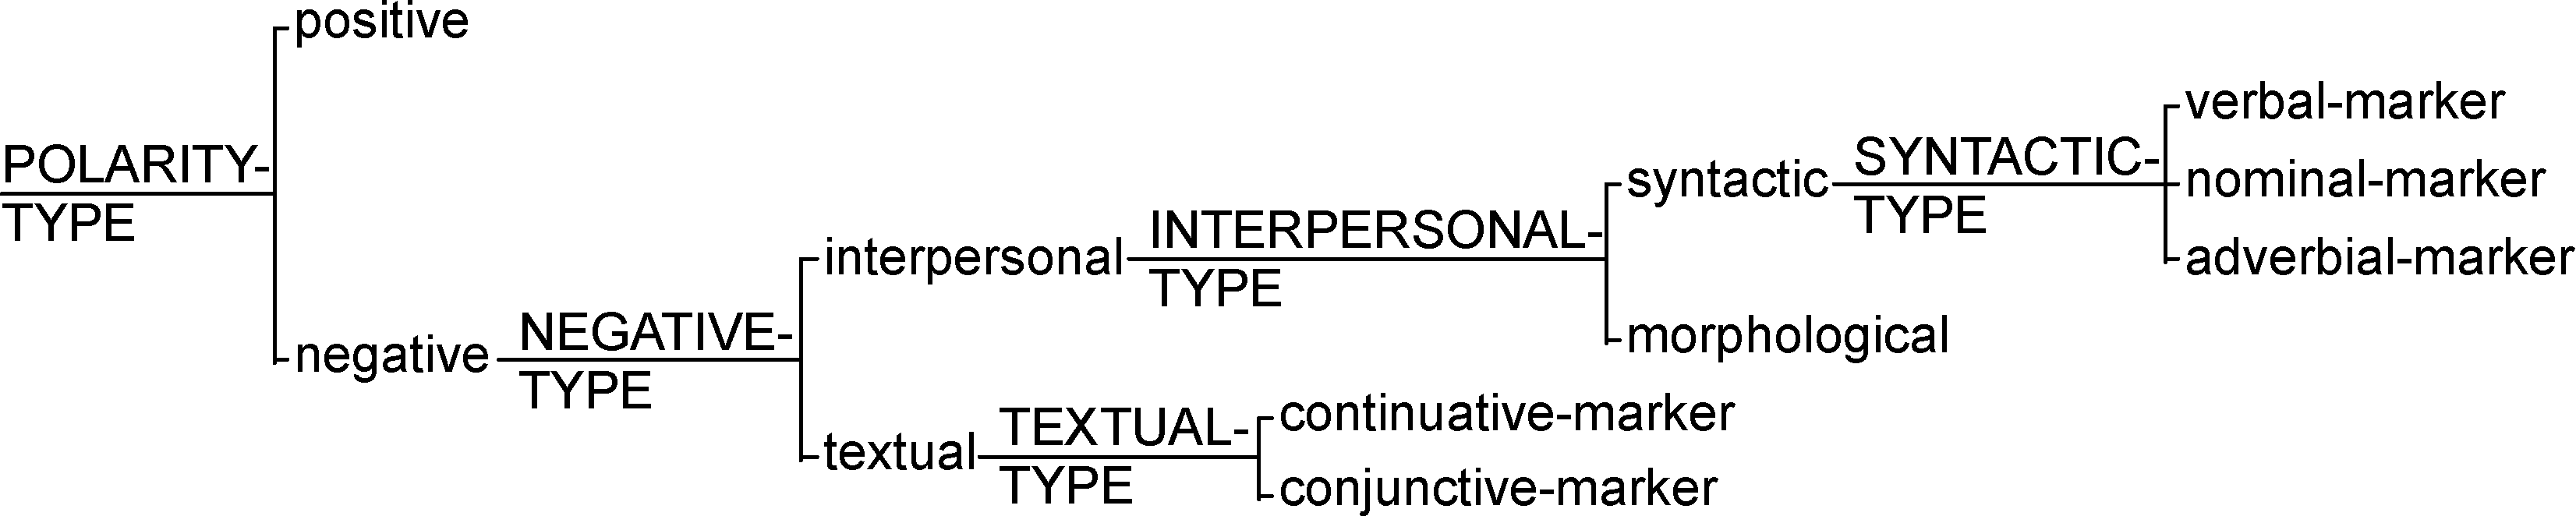
\includegraphics[width=\textwidth]{Figures/SFL-grammar/polarity-system.pdf}
\caption{Polarity System}
\label{fig:polarity1}
\end{figure}

Take for instance the POLARITY system in Figure \ref{fig:polarity1}. Its default selection is \textit{positive} feature unless there is a negative marker. So we must asses NEGATIVE-TYPE system to resolve POLARITY system. But NEGATIVE-TYPE also must be postponed because we do not know if there is a negative marker unless we run tests for each marker type (i.e. presence of a ``no'' particle, negative subject or adjunct etc.). So we postpone selection decision and activate further the INTERPERSONAL-TYPE and TEXTUAL-TYPE systems and base the assessment on the selections yielded by the latter two systems. The same story is with INTERPERSONAL-TYPE which can make selections based on what SYNTACTIC-TYPE system yields. If SYNTACTIC-TYPE and TEXTUAL-TYPE systems yield no selection then we return recursively to INTERPERSONAL-TYPE and to NEGATIVE-TYPE and yield no selection in those systems as well. However if, for instance, \textit{verbal-marker} is detected in the clause then the \textit{syntactic} feature is yielded by the INTERPERSONAL-TYPE and \textit{interpersonal} by the NEGATIVE-TYPE and thus \textit{negative} is yielded by the POLARITY-TYPE. 

Moreover the negative markers can be of various types and more than one can occur simultaneously without any interdependence between them so the algorithm needs to check presence of every type of negative marker i.e. verbal, nominal adverbial, conjunctive and continuative markers. 

That being said the intermediary systems and features i.e. interpersonal, textual, syntactic, morphological are there for the classification purpose only and do not carry any particular algorithmic value making the network from Figure \ref{fig:polarity1} reducible to the one in Figure \ref{fig:polarity1-condensed}. 

\begin{figure}[H]
\centering
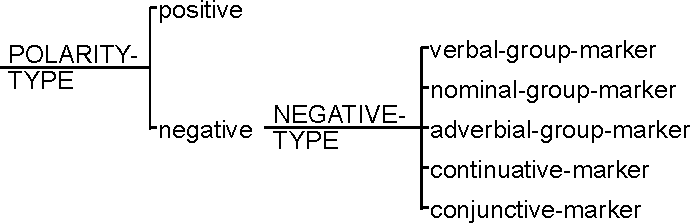
\includegraphics[width=0.6\textwidth]{Figures/SFL-grammar/polarity-condensed.pdf}
\caption{Condensed Polarity System}
\label{fig:polarity1-condensed}
\end{figure}

Execution of system networks is subject to constituent \textit{enrichment phase} of the parsing algorithm. Reducing the POLARITY network to the one in Figure \ref{fig:polarity1-condensed} would lead to loss of information which may be relevant for choice-making in other systems (e.g. MODALITY) so it is useful to expand the selection set with dependent features to achieve feature rich constituents.

%TODO
\section{Discussion}
This chapter describes the elemental data structure and the kinds of operations that current implementation applies to generate the SFG parse structures. It lays down the foundations for next chapter which focuses on the parsing pipeline and algorithms. 

A central theme covered here are the graphs and graph patterns. They play the key role in identifying grammatical features in dependency and constituency structures. They are also excellent candidate for expressing \textit{systemic realization rules}. 

Robin Fawcett recurrently emphasises the role of realization rules in the composition of system networks. He often stresses ``no system networks without realization rules''. They are important because they formally express ways in which a feature is identified or realised. It is the \textit{instantiation} process that in Halliday's words ``is the relation between a semiotic system and the \textit{observable} events or `acts' of meaning'' \citep[emphasis added]{Halliday2003-systemic-theory}. The realisation rules for a systemic feature are the statement of operations through which that feature contributes to the structural configuration (that is being either generated or recognised) \citep[p.86]{Fawcett2000}.

It is not easy however for linguists and grammarians to provide such statements for the systemic features. Doing so means an explicit formalisation of grammar on top of charting the systemic composition and dependencies which is already a challenging task in its own. The realisation rules most of the time remain in the minds of the interpreters who can recognise a feature when it occurs. Adding the formal specification of the realisation rule requires tools for consistency checking with respect to the rest of the grammar and large corpus query tool to test various rule hypotheses. 

Moreover the expression of rules is proposed in terms of atomic operations such as lexify, preselect, insert, order, etc. Which may not always be fully transparent to the grammarian. Expressing realization rules as operations contextualised in fragments of parse structure is a promising way to ease the grammar authoring process. They could then be used directly by the parser to recognise such structures making the corpus annotation and grammar construction an in-parallel evolving process.

The data structures and operations described in this chapter can be a suitable approach to address the problem of missing realisation rules from the system networks. To do so however requires creation of a system network authoring tool (such as the one available in UAM Corpus Tool \citep{ODonnell2008a}) which besides systemic network editor should contain also a graph pattern editor allowing association of graph patterns to systemic features and . 

In current parser the pattern graphs are represented as compositions of Python dictionaries and lists such as the one below.
%* The Patterns are written as python data structures thus not very user friendly, an editor would be much more helpful
\begin{Verbatim}[fontsize=\relsize{-2}]
{
    NODES: {  
        "cl": [
            {C_TYPE: 'clause', 
             VOICE: ACTIVE},
            {CONFIGURATION: ['two-role-action', ['Ag', 'Ra', 'Cre']], }],
        'pred': [
            {C_TYPE: [PREDICATOR, PREDICATOR_FINITE], }, 
            {VERB_TYPE: "main", PROCESS_TYPE: 'two-role-action'} ],
        'subj': [
            {C_TYPE: SUBJECT, }, 
            {PARTICIPANT_ROLE: 'Ag'}],
        'compl1': [
            {C_TYPE: [COMPLEMENT, COMPLEMENT_DATIVE], },
            {PARTICIPANT_ROLE: 'Ra'}],
        'compl2': [
            {C_TYPE: [COMPLEMENT, COMPLEMENT_ADJUNCT, ], },
            {PARTICIPANT_ROLE: 'Cre'}],
    },
    EDGES: [
    ['cl', 'pred', None], 
    ['cl', 'subj', None], 
    ['cl', 'compl1', None], 
    ['cl', 'compl2', None],]
}
\end{Verbatim}

This Python dictionary contains two top keys: NODES defined as  with node identifiers each associated with a set of systemic features and EDGES defined as a list with three tuples of source, target and eventually a dictionary of features. The nodes contain a list of two dictionaries. The first dictionary enlists the features that the backbone structure should already carry, and against which the pattern matching is performed. The second dictionary contains the set of features that the node shall receive in case of a successful match of the entire pattern. 

Writing such structures is cumbersome and requires in depth knowledge of the parser and employed system networks therefore the need for an editor is even higher. Unfortunately building such an editor is out of the scope of the current work and is among the priorities in the future developments just as switching to better technology for working with graphs such as Semantic Web suite of tools. This and other future work are described in the Section \ref{sec:future-work}.

In the next chapter I describe the parsing pipeline and how each step is implemented starting from Stanford dependency graph all the way down to a rich constituency systemic functional parse structure.